%\chapter{Real Data}
%Finally, we also performed inference on a real FMRI scan. The scanner we used...
%... more specifics...

% TODO include single?
%Before performing tests on a full image, I the particle filter
%on regions deemed active and inactive by statistical parametric mapping
%(SPM). This served the purpose of adjusting the priors as well as the 
%preprocessing based on real world signals. This was actually done before
%the simulations, and then results were carried back the simulations 
%to check consistency.
%After work adjusting parameters, most importantly the weighting function and the 
%priors, particle filter was applied to every voxel in an FMRI image.
%The results of this large scale analysis was a parameter map which was
%then used to calculate normalized square-root MSE image. 
%
%\section{Single-Voxel Analysis}
%The choice of a prior, as discussed previously, is extremely important. While a
%prior may have the potential to give good results, being a monte-carlo algorithm
%there is the possibility for inconsistencies. Thus, increasing the variance
%of the time-constants may allow additional flexibility, it will also cause
%additional model variance. Before running on a full volume I adjusted the 
%prior to ensure that the same input would give the same output 100 times in a 
%row. While this may seem like a given, with a random drawing of the prior,
%this can be difficult. Case in point, the exact same algorithm run twice
%with the time constants all having standard deviations of $.35$ resulted in two
%very different fits, shown in \autoref{fig:badfit_param1}.
%
%\begin{figure}
%\subfigure{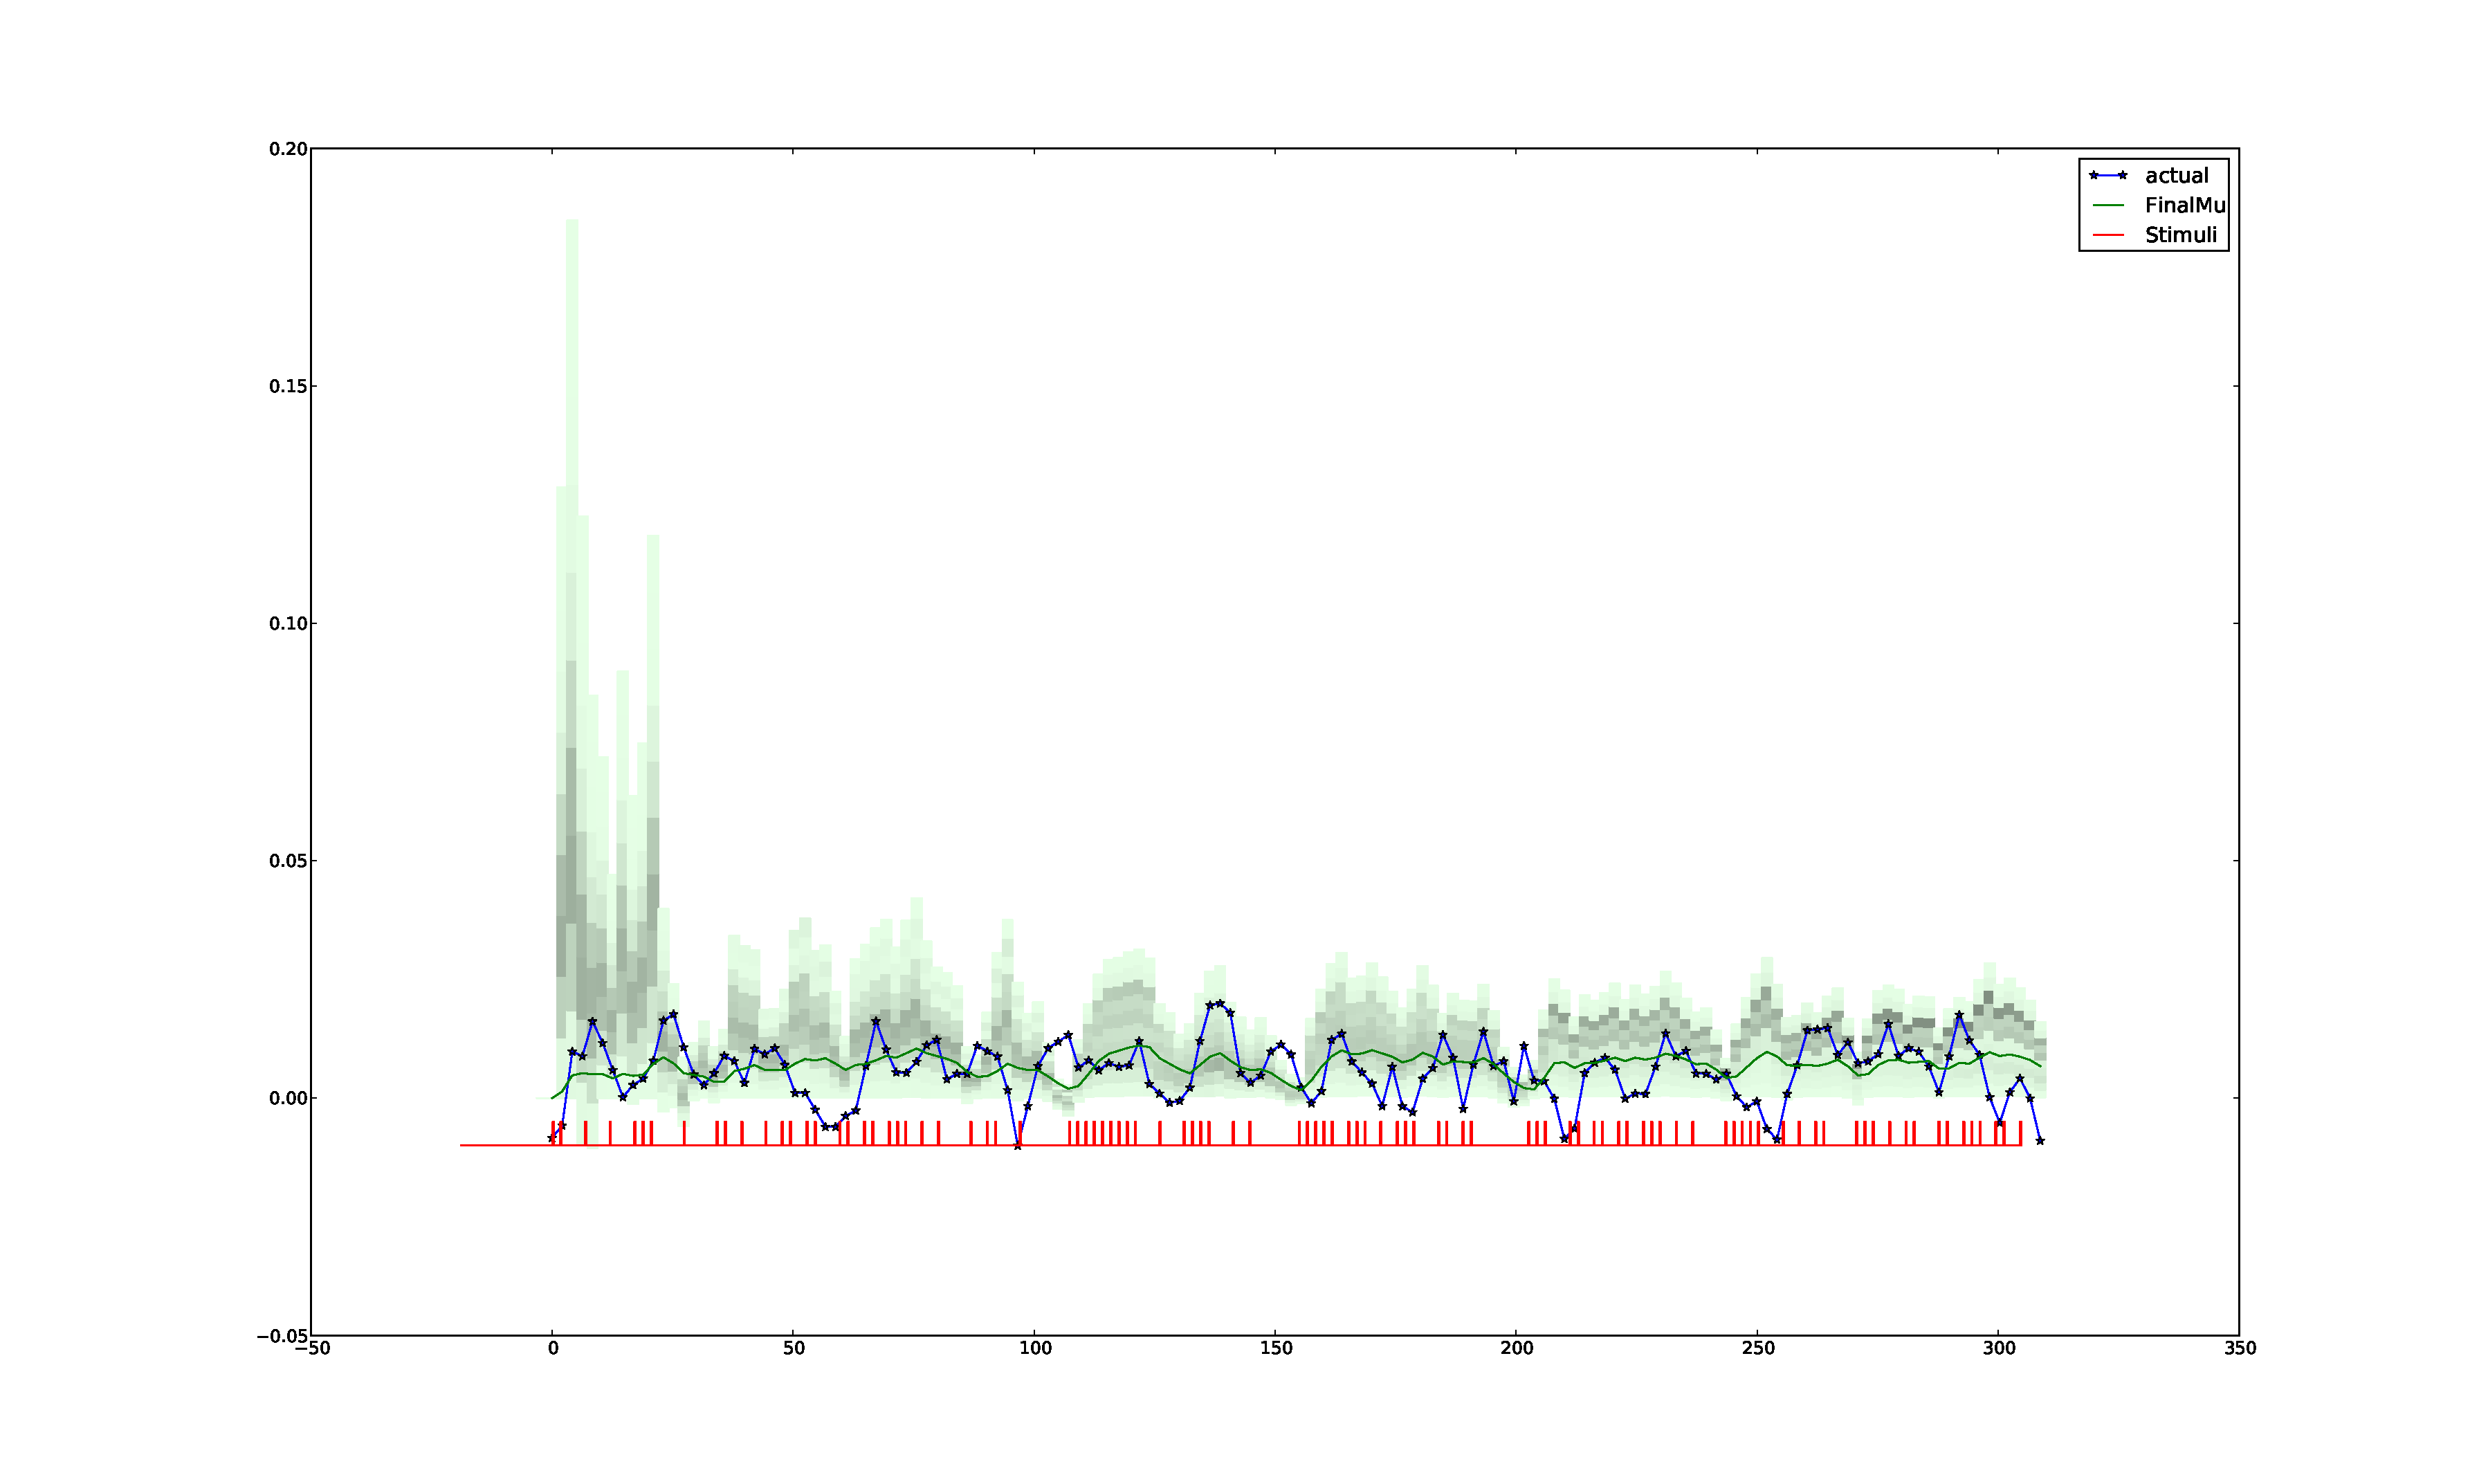
\includegraphics[clip=true,trim=6cm 2cm 6cm 3.5cm,width=17cm]{images/badfit_param1}}
%\subfigure{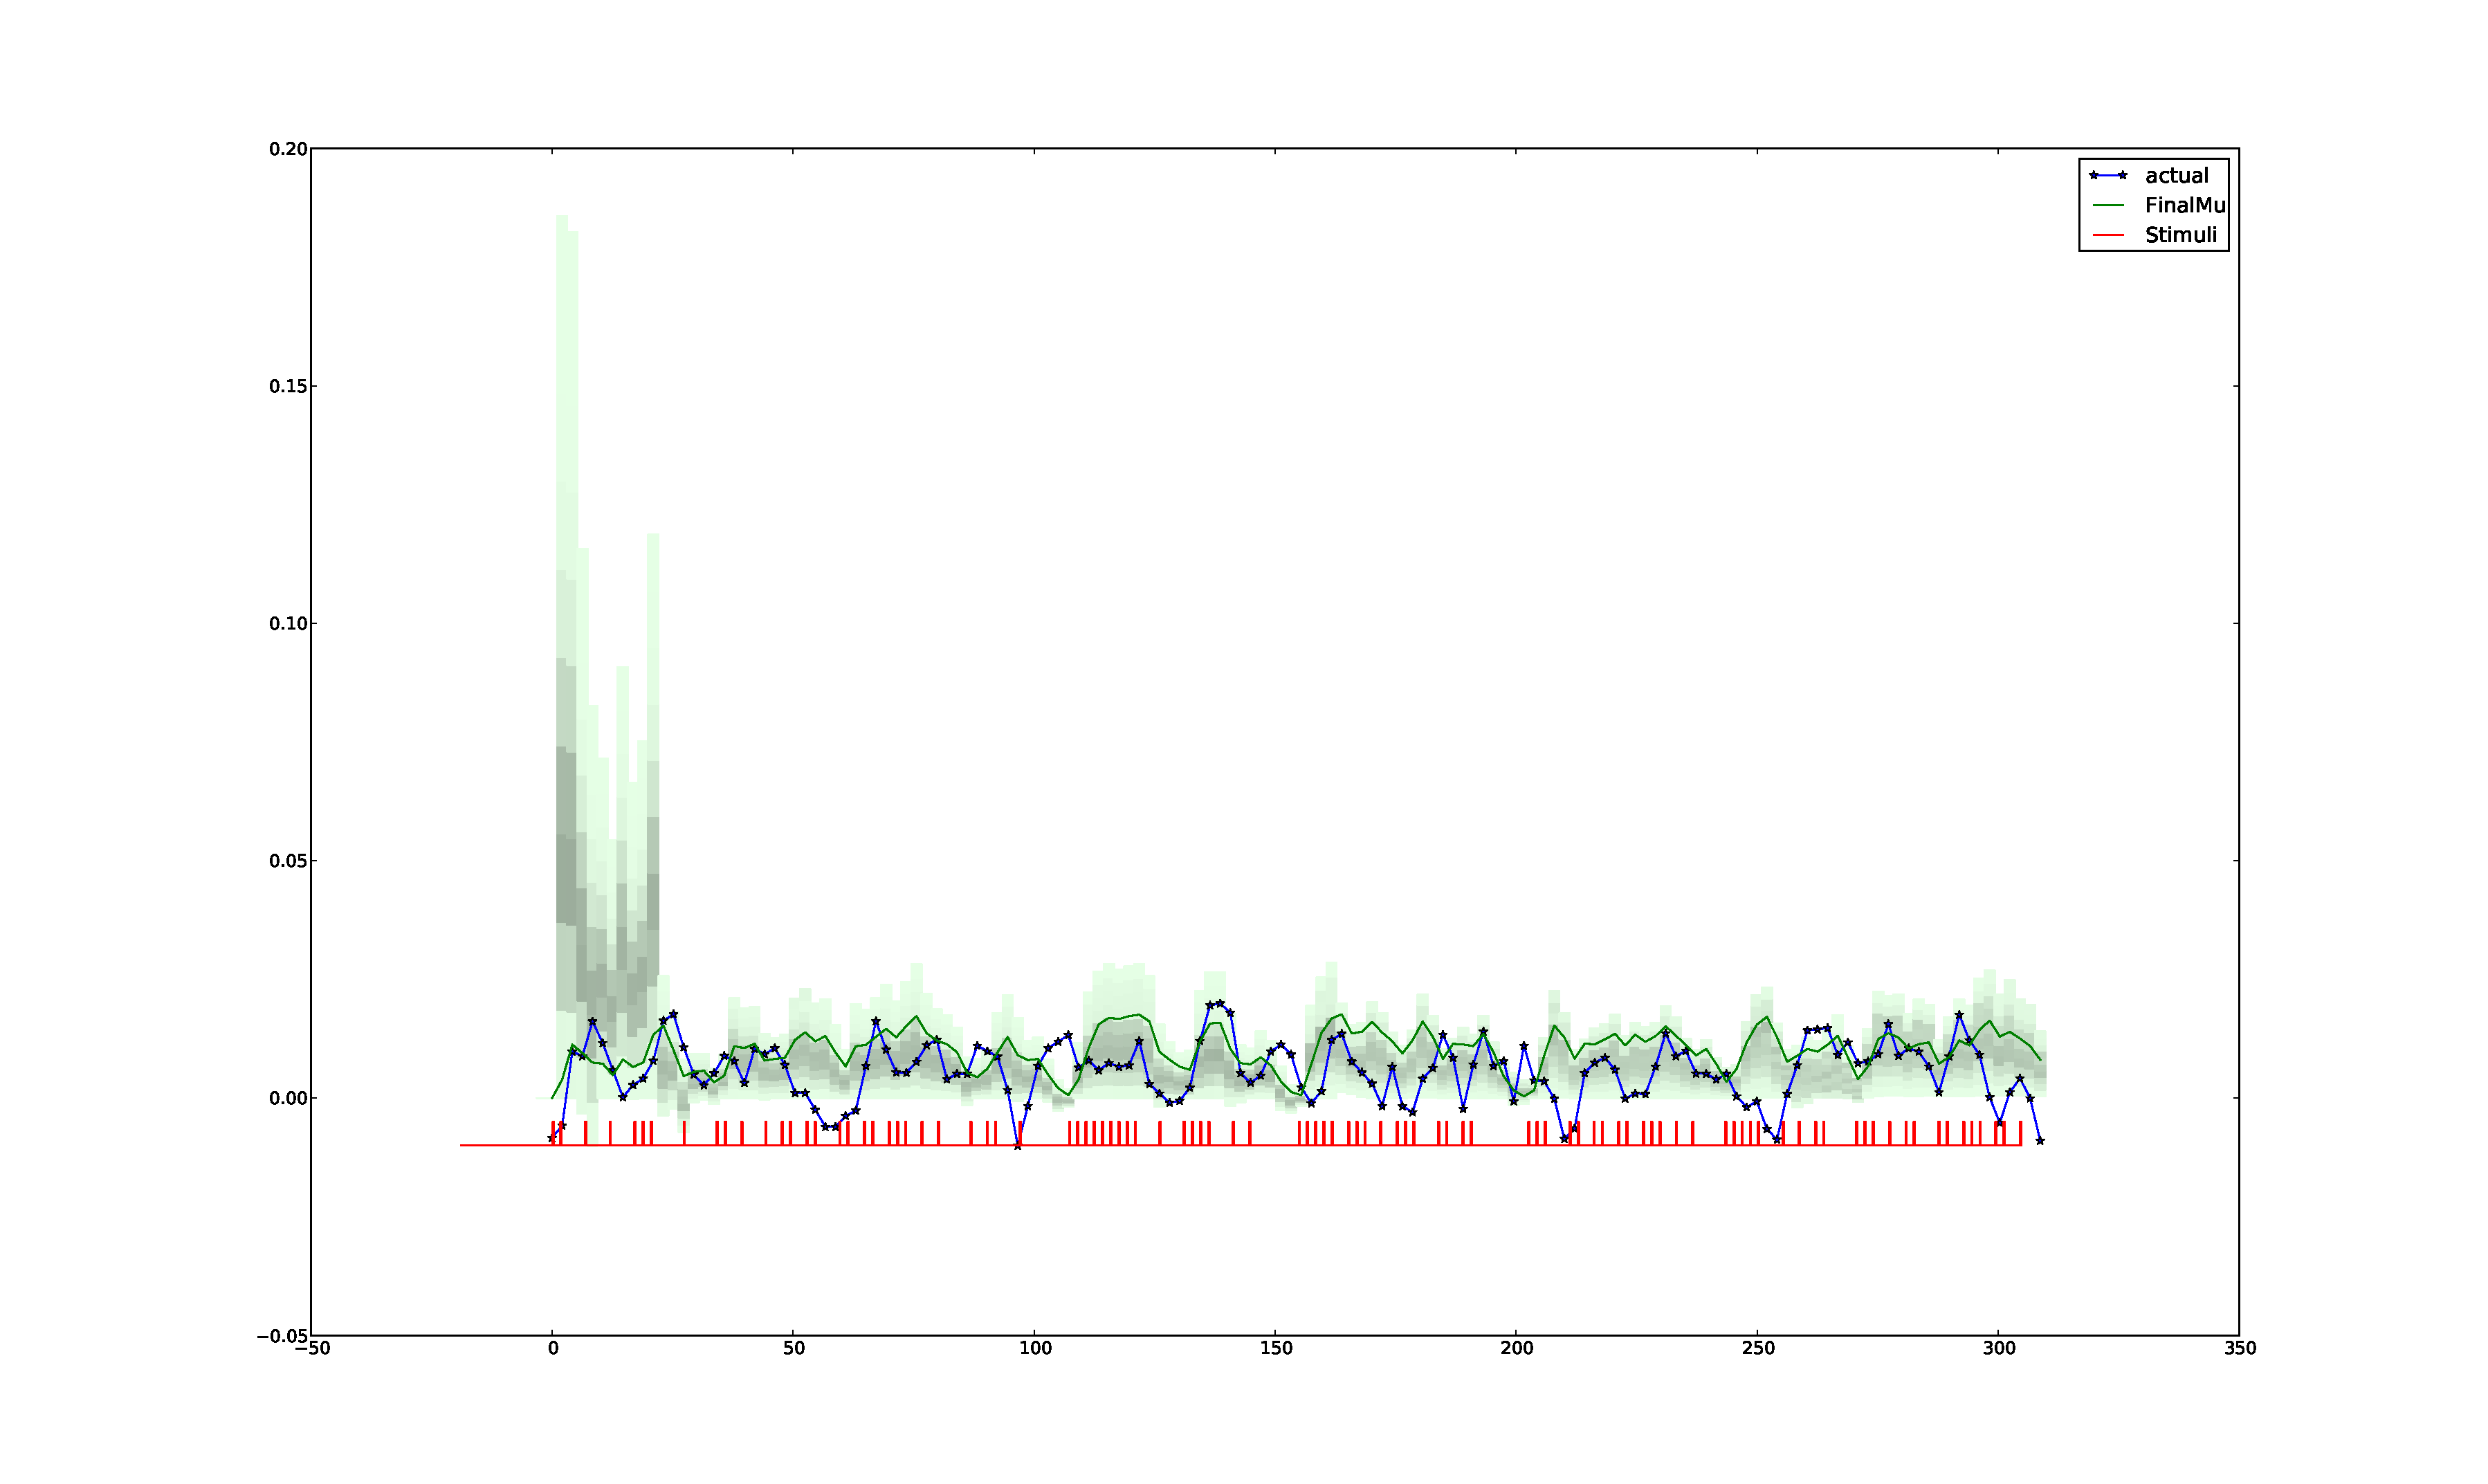
\includegraphics[clip=true,trim=6cm 2cm 6cm 3.5cm,width=17cm]{images/goodfit_param1}}
%\caption{The same priors gave rise to both fits.}
%\label{fig:badfit_param1}
%\end{figure}
%
%For this reason, I actually lowered the standard deviations of the time
%constants to prevent over-smoothing. This resulted in more consistent,
%though potentially slightly worse fits, two examples of which are 
%shown in \autoref{fig:param2_var}. 
%
%\begin{figure}
%\subfigure{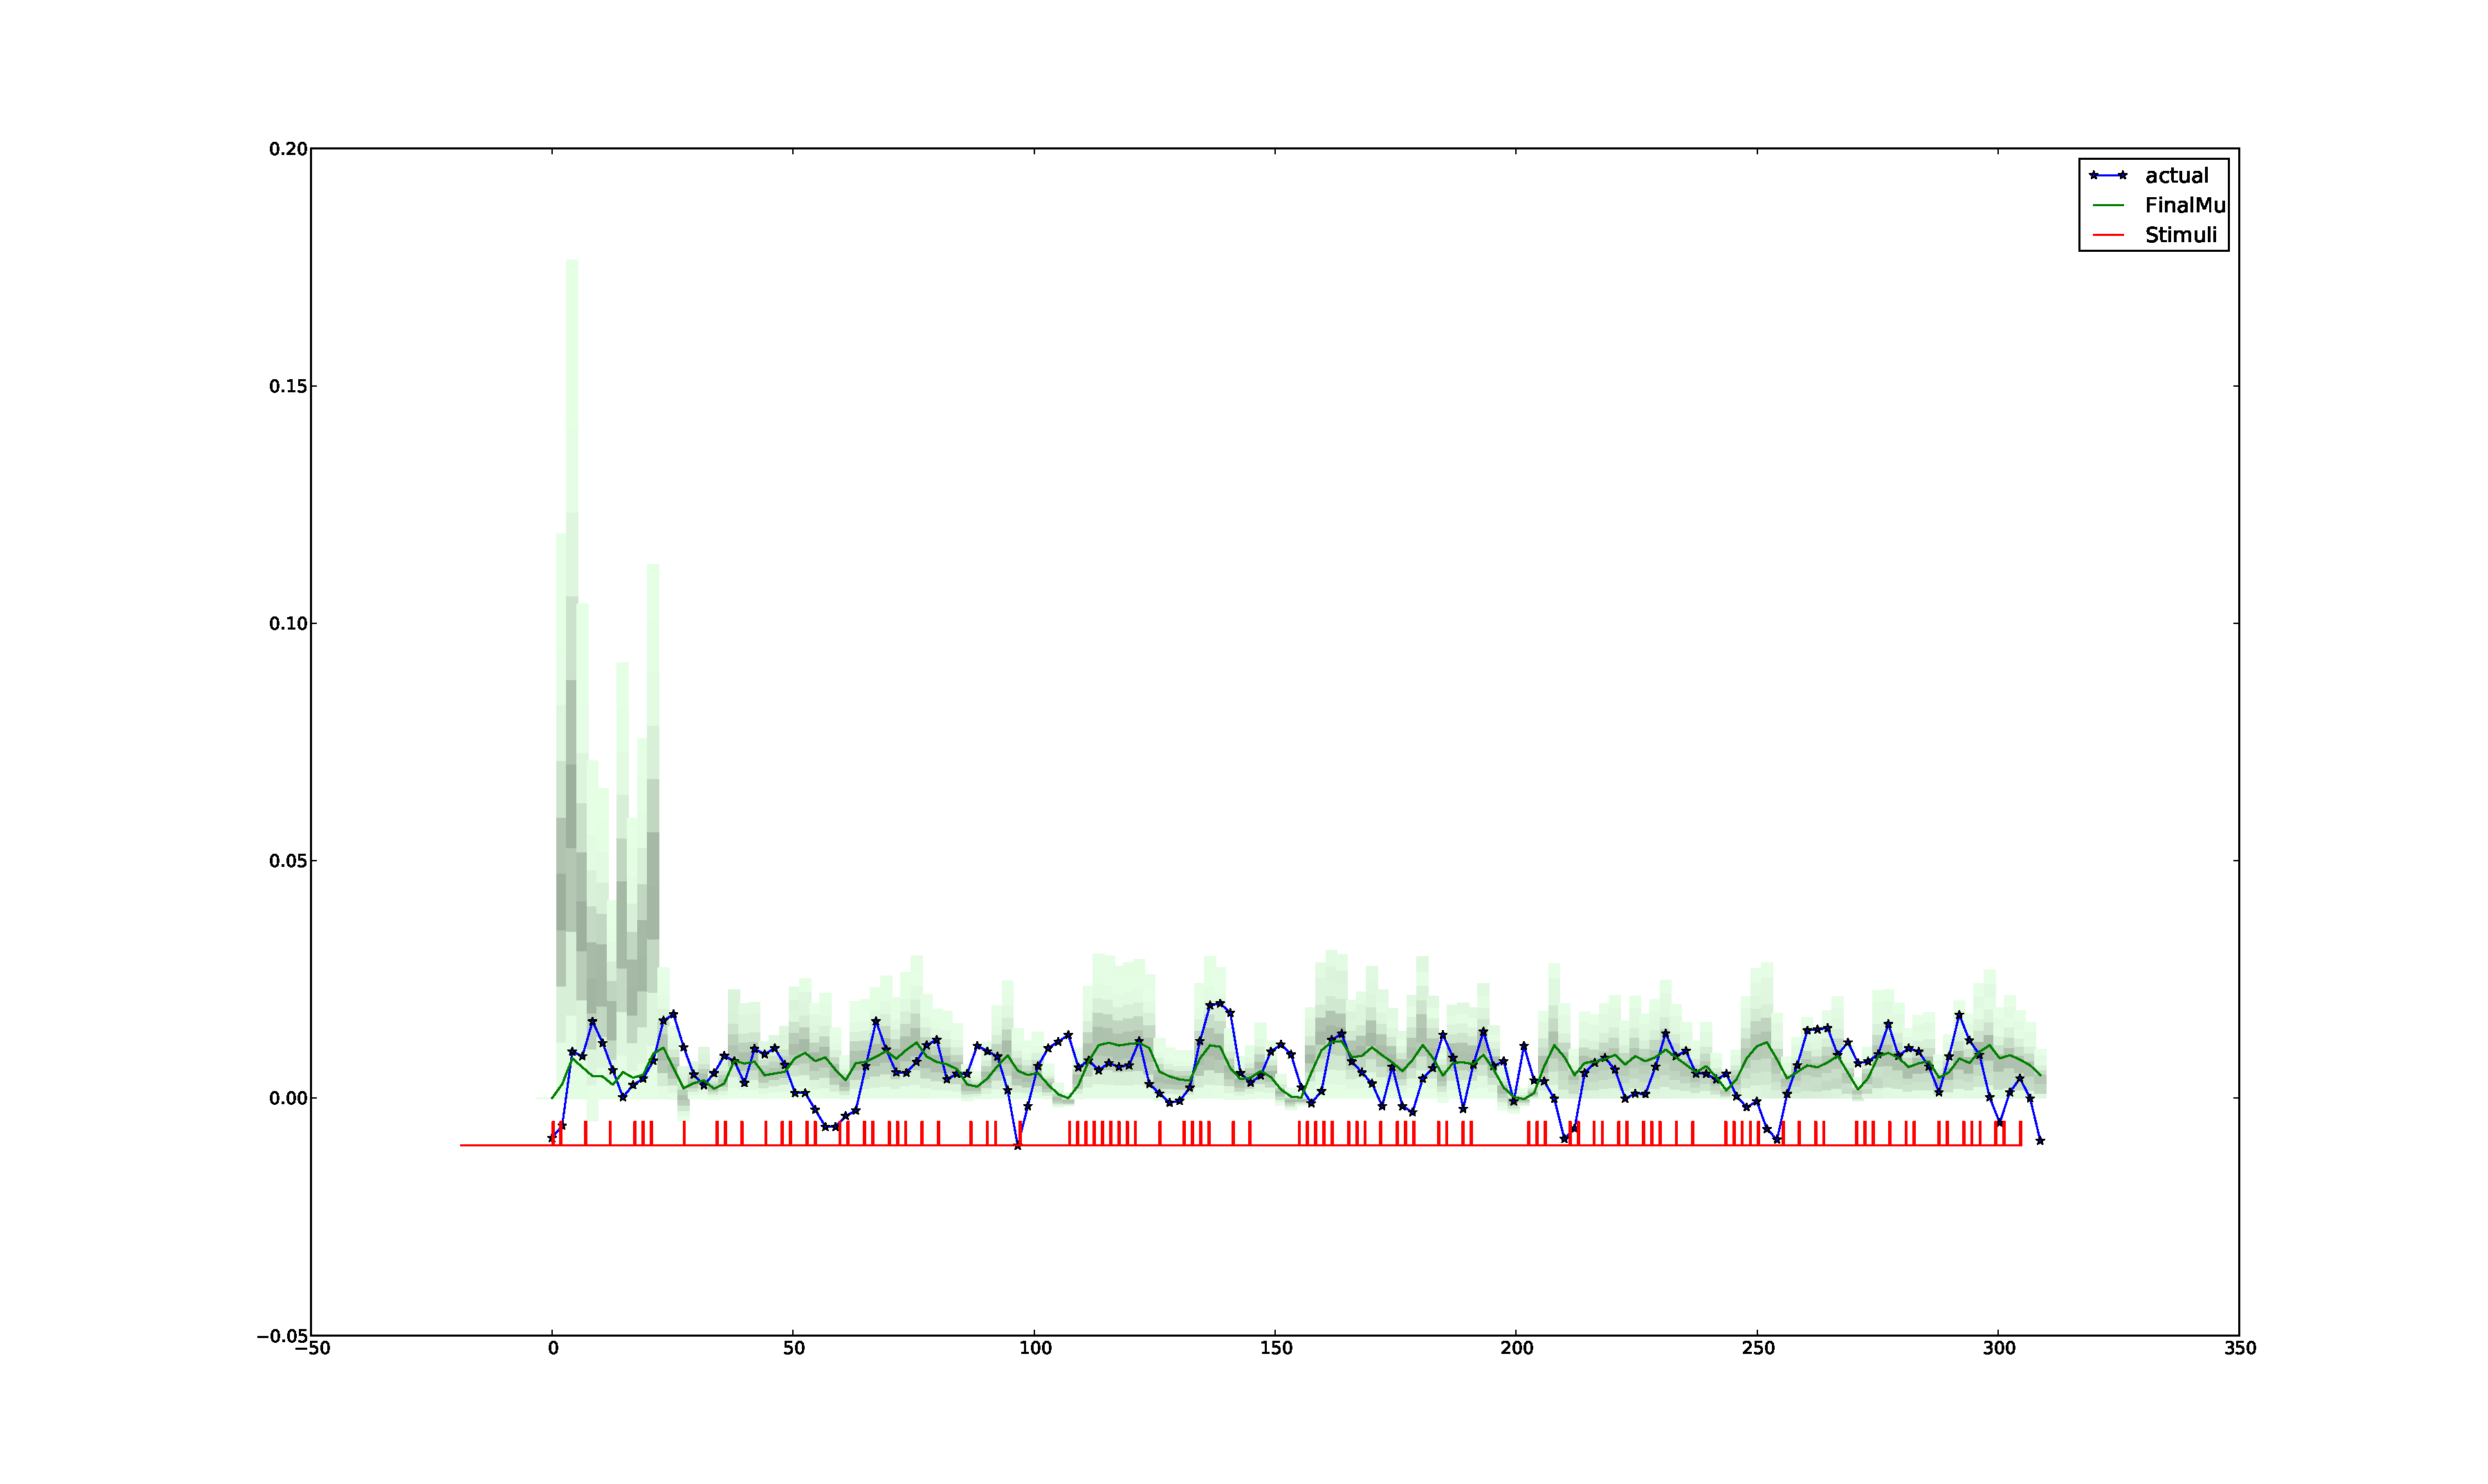
\includegraphics[clip=true,trim=6cm 2cm 6cm 3.5cm,width=17cm]{images/param2a}}
%\subfigure{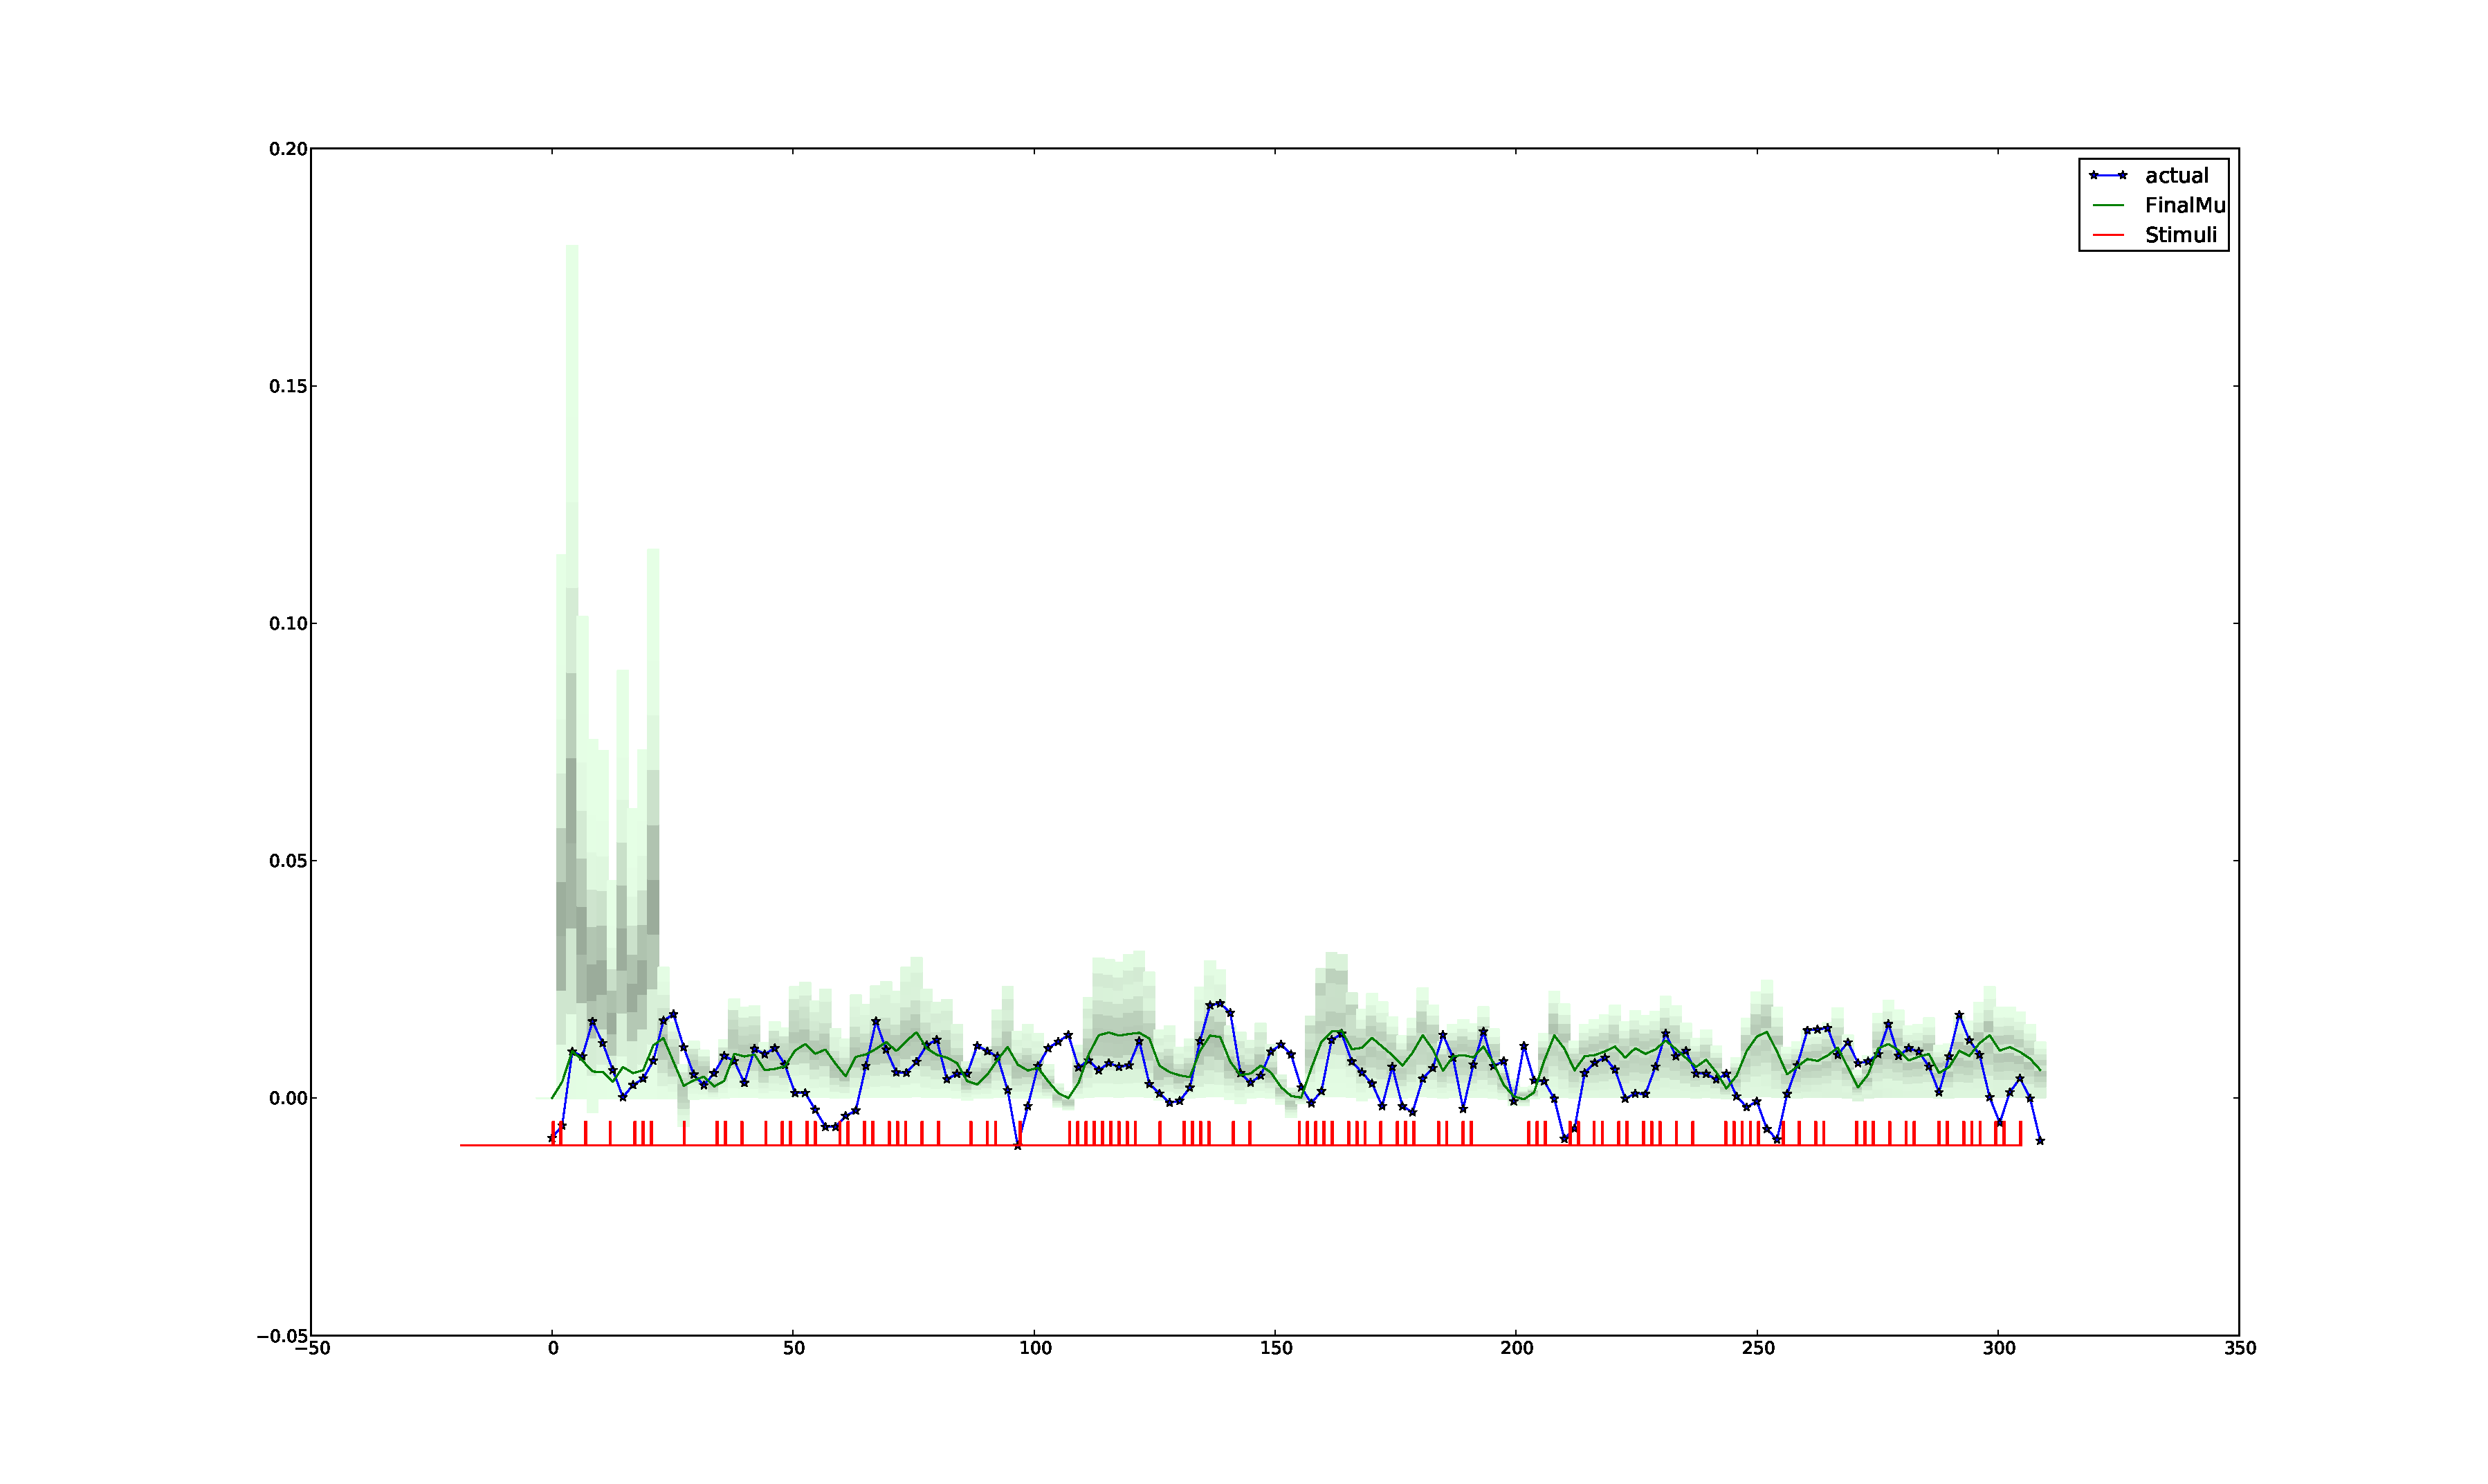
\includegraphics[clip=true,trim=6cm 2cm 6cm 3.5cm,width=17cm]{images/param2b}}
%\caption{A poor fit, using the same parameters as }
%\label{fig:param2_var}
%\end{figure}
%
%todo: stats of the 100 fits?
%
%\section{Single Time-Series Simulation}
%
\chapter{Real Data}
\label{sec:RealData}
Modeling the BOLD response is of course not of much use if it is only done in a 
single voxel. Although this algorithm will hopefully lead to more novel methods 
of analysis, the standard use for modeling the BOLD signal is to locate activation.
Activation is essentially defined as areas where the input seems to directly drive
the BOLD response, as opposed to there being intermediate factors controlling it. 
Once areas where the BOLD 
model may be accurately estimated are found, integrating the model will allow for accurate
estimation of the state between measurements, which could then be used for more 
advanced analysis, for instance of areas that are being driven by other brain regions.
It all begins with localizing the first activation regions in the
chain. Therefore this section compares the output of the particle filter 
with conventional SPM. 

In reality, the statistical parametric mapping method is very different from the 
particle filter algorithm described in this work.
SPM preprocesses the image by spatially smoothing the FMRI image (in this section 
SPM8 was used with an $8mm x 8mm x 8mm$ Gaussian kernel), whereas
this is not done in the particle filter algorithm. Additionally, a spline
was used to de-trend, rather than SPM8's high pass filter (with a cut
off based on a globally estimated autocorrelation). Thus the preprocessing pipelines 
are different; but the output of SPM8 is also different. Whereas SPM outputs
a t-statistic for each voxel, the output 
of the particle filter is a posterior probability distribution of the parameters
at every voxel. To validate the quality of the particle filter results though
it is necessary to compare the location and fit of the particle filter parameter
mapping with SPM's T-score map. 

\section{Results}

The results from SPM8 are shown in \autoref{fig:hm_canon_spm}, and the results from 
the particle filter are shown in \autoref{fig:hm_canon_pfilter}. Note again that the
output is actually a different scale. Whereas the levels in the SPM map are T-Scores
indicating the probability that the result cannot be explained from a random signal,
the result of the particle filter is simply a normalized square-root of the mean-squared-
residual. Thus, lower is better, and zero is a perfect fit in the particle filter whereas
infinity is a perfect fit in \autoref{fig:hm_canon_spm}. Note that it would seem that there
are quite a few dispersed areas with decent fits in \autoref{fig:hm_canon_pfilter}. Also,
interestingly the lowest error was just above $.7$. 
For the sake of completeness \autoref{fig:hm_canon_pfilter85} shows the same image but
thresheld at $.85$ rather than $1$. Obviously this image seems like a closer match to
the results of SPM, however, the results of \autoref{fig:hm_canon_pfilter} are interesting.

\begin{figure}[H]
\subfigure[]{\label{fig:hm_spm} 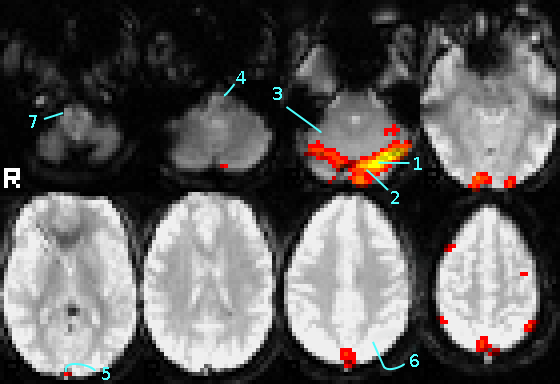
\includegraphics[scale=.66]{images/spm_hm}}
\subfigure[]{\label{fig:hm_canon_spm_x} 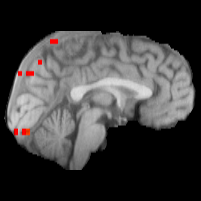
\includegraphics[scale=.85]{images/spm_hm_x}}
\subfigure[]{\label{fig:hm_canon_spm_y} 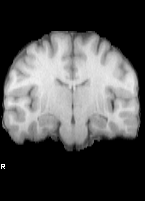
\includegraphics[scale=.85]{images/spm_hm_y}}
\subfigure[]{\label{fig:hm_canon_spm_z} 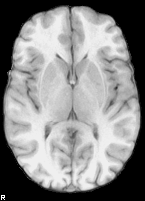
\includegraphics[scale=.85]{images/spm_hm_z}}
\subfigure{\label{fig:scale_spm} 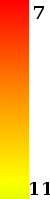
\includegraphics[scale=.3]{images/scale1}}
\caption{Sagittal, coronal and axial slices of SPM results (\autoref{fig:hm_canon_spm_x} \autoref{fig:hm_canon_spm_y} 
         \autoref{fig:hm_canon_spm_x}), as well as a series of axial slices, \autoref{fig:hm_spm}. Units
         of activation are in Student's T-scores. Higher indicates higher assurance that the signal cannot
         have occurred through noise alone.}
\label{fig:hm_canon_spm}
\end{figure}

\begin{figure}[H]
\subfigure[]{\label{fig:hm_pfilter} 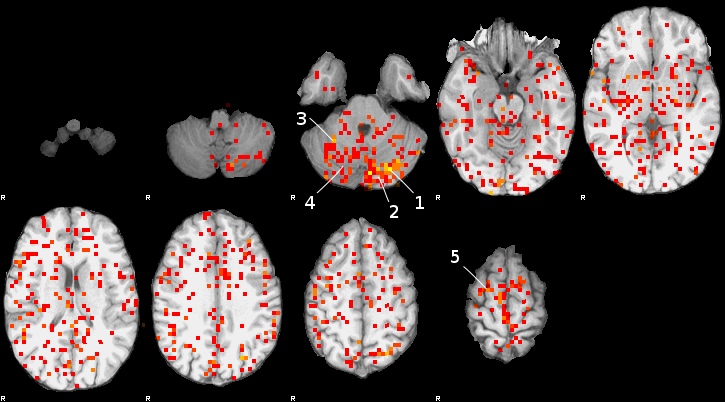
\includegraphics[scale=.66]{images/pfilter_hm}}
\subfigure[]{\label{fig:hm_canon_pfilter_x} 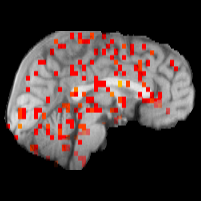
\includegraphics[scale=.85]{images/pfilter_hm_x}}
\subfigure[]{\label{fig:hm_canon_pfilter_y} 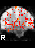
\includegraphics[scale=.85]{images/pfilter_hm_y}}
\subfigure[]{\label{fig:hm_canon_pfilter_z} 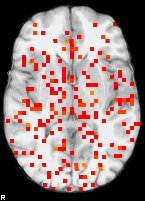
\includegraphics[scale=.85]{images/pfilter_hm_z}}
\subfigure{\label{fig:scale_pfilter} 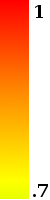
\includegraphics[scale=.3]{images/scale2}}
\caption{Sagittal, coronal and axial slices of SPM results (\autoref{fig:hm_canon_pfilter_x} \autoref{fig:hm_canon_pfilter_y} 
         \autoref{fig:hm_canon_pfilter_x}), as well as a series of axial slices, \autoref{fig:hm_pfilter}. 
         Units of match is normalized error. The lowest (best) levels were $.7$,
         whereas the worst levels could go higher than 100 (not shown).}
\label{fig:hm_canon_pfilter}
\end{figure}

\begin{figure}[H]
\subfigure[]{\label{fig:hm_pfilter85} 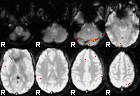
\includegraphics[scale=.66]{images/pfilter85_hm}}
\subfigure[]{\label{fig:hm_canon_pfilter85_x} 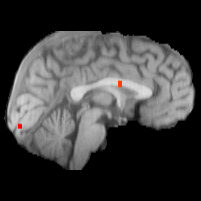
\includegraphics[scale=.85]{images/pfilter_hm85_x}}
\subfigure[]{\label{fig:hm_canon_pfilter85_y} 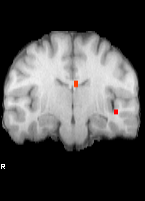
\includegraphics[scale=.85]{images/pfilter_hm85_y}}
\subfigure[]{\label{fig:hm_canon_pfilter85_z} 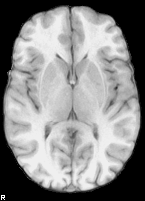
\includegraphics[scale=.85]{images/pfilter_hm85_z}}
\subfigure{\label{fig:scale_pfilter85} 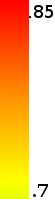
\includegraphics[scale=.3]{images/scale3}}
\caption{Sagittal, coronal and axial slices of SPM results (\autoref{fig:hm_canon_pfilter_x} \autoref{fig:hm_canon_pfilter_y} 
         \autoref{fig:hm_canon_pfilter_x}), as well as a series of axial slices, \autoref{fig:hm_pfilter}. 
         Units of match is normalized $\sqrt{MSE}$. The lowest (best) levels were $.7$,
         whereas the worst levels could go higher than 100 (not shown).}
\label{fig:hm_canon_pfilter85}
\end{figure}

\begin{figure}
\subfigure[Particle Filter]{\label{fig:comp1pfilter} 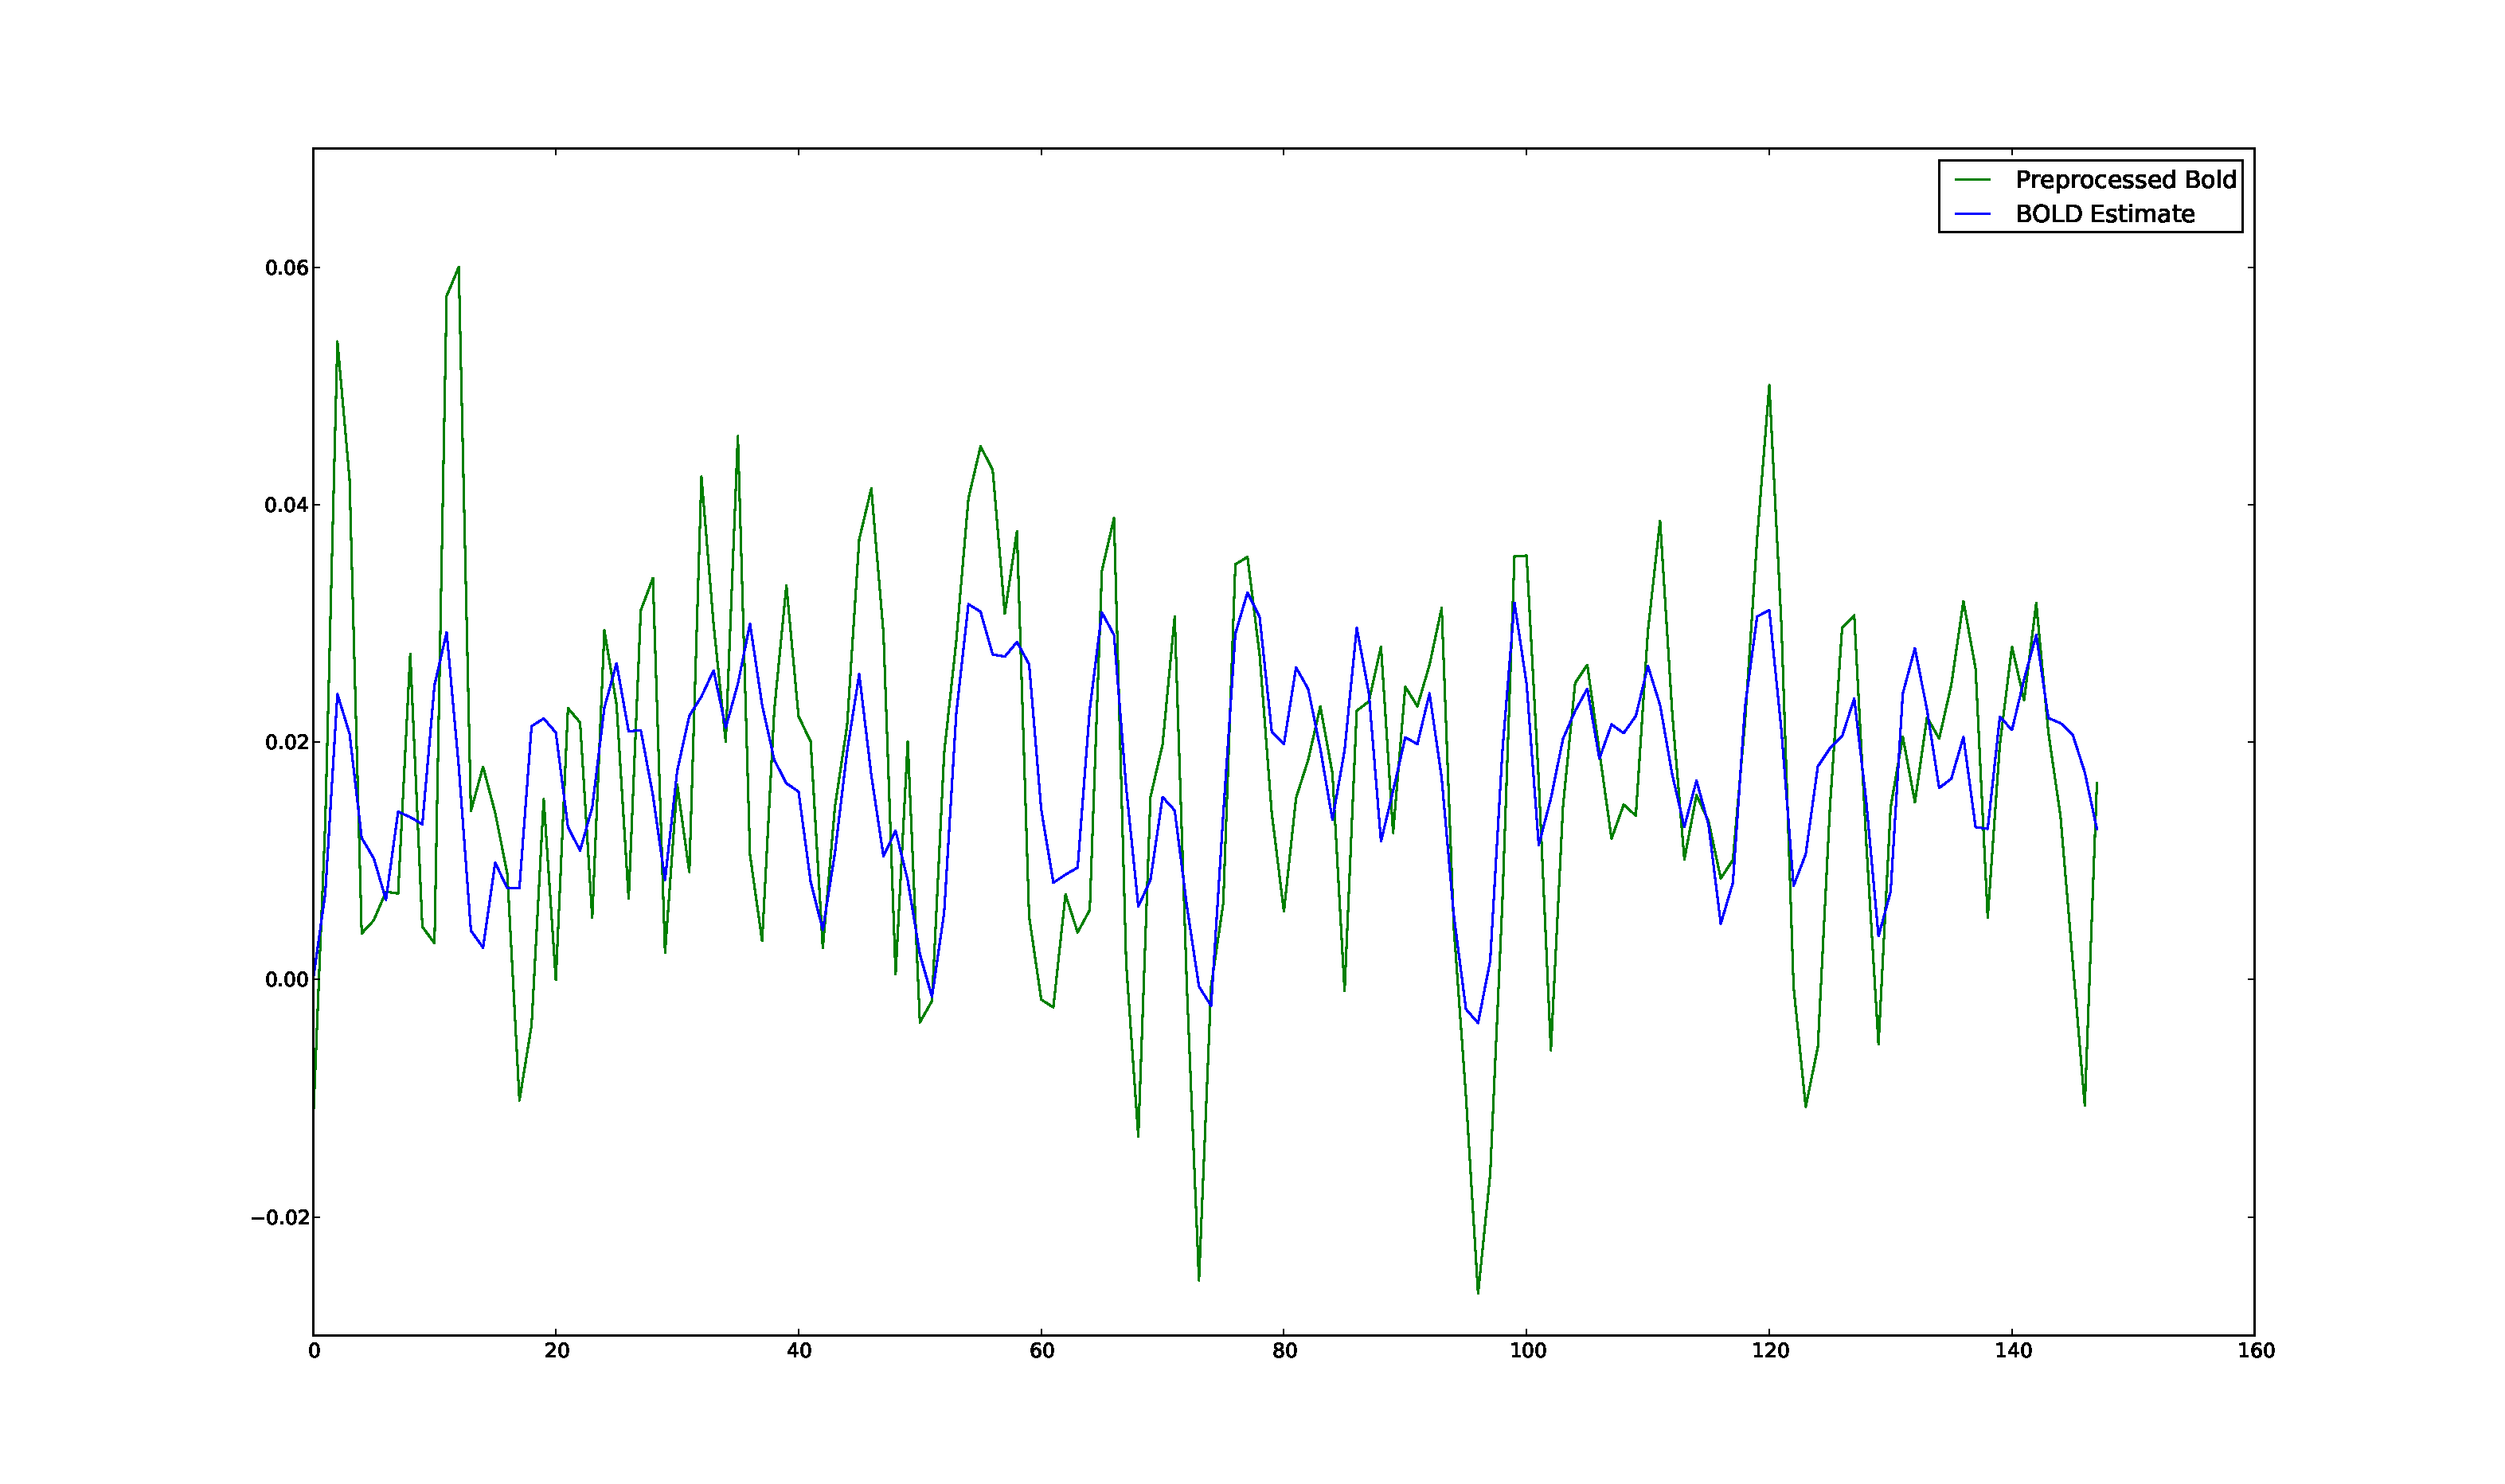
\includegraphics[clip=true,trim=5cm 1cm 4cm 1cm,width=15cm]{images/1_pfilter_37_14_7}}\\
\subfigure[SPM]{\label{fig:comp1spm} 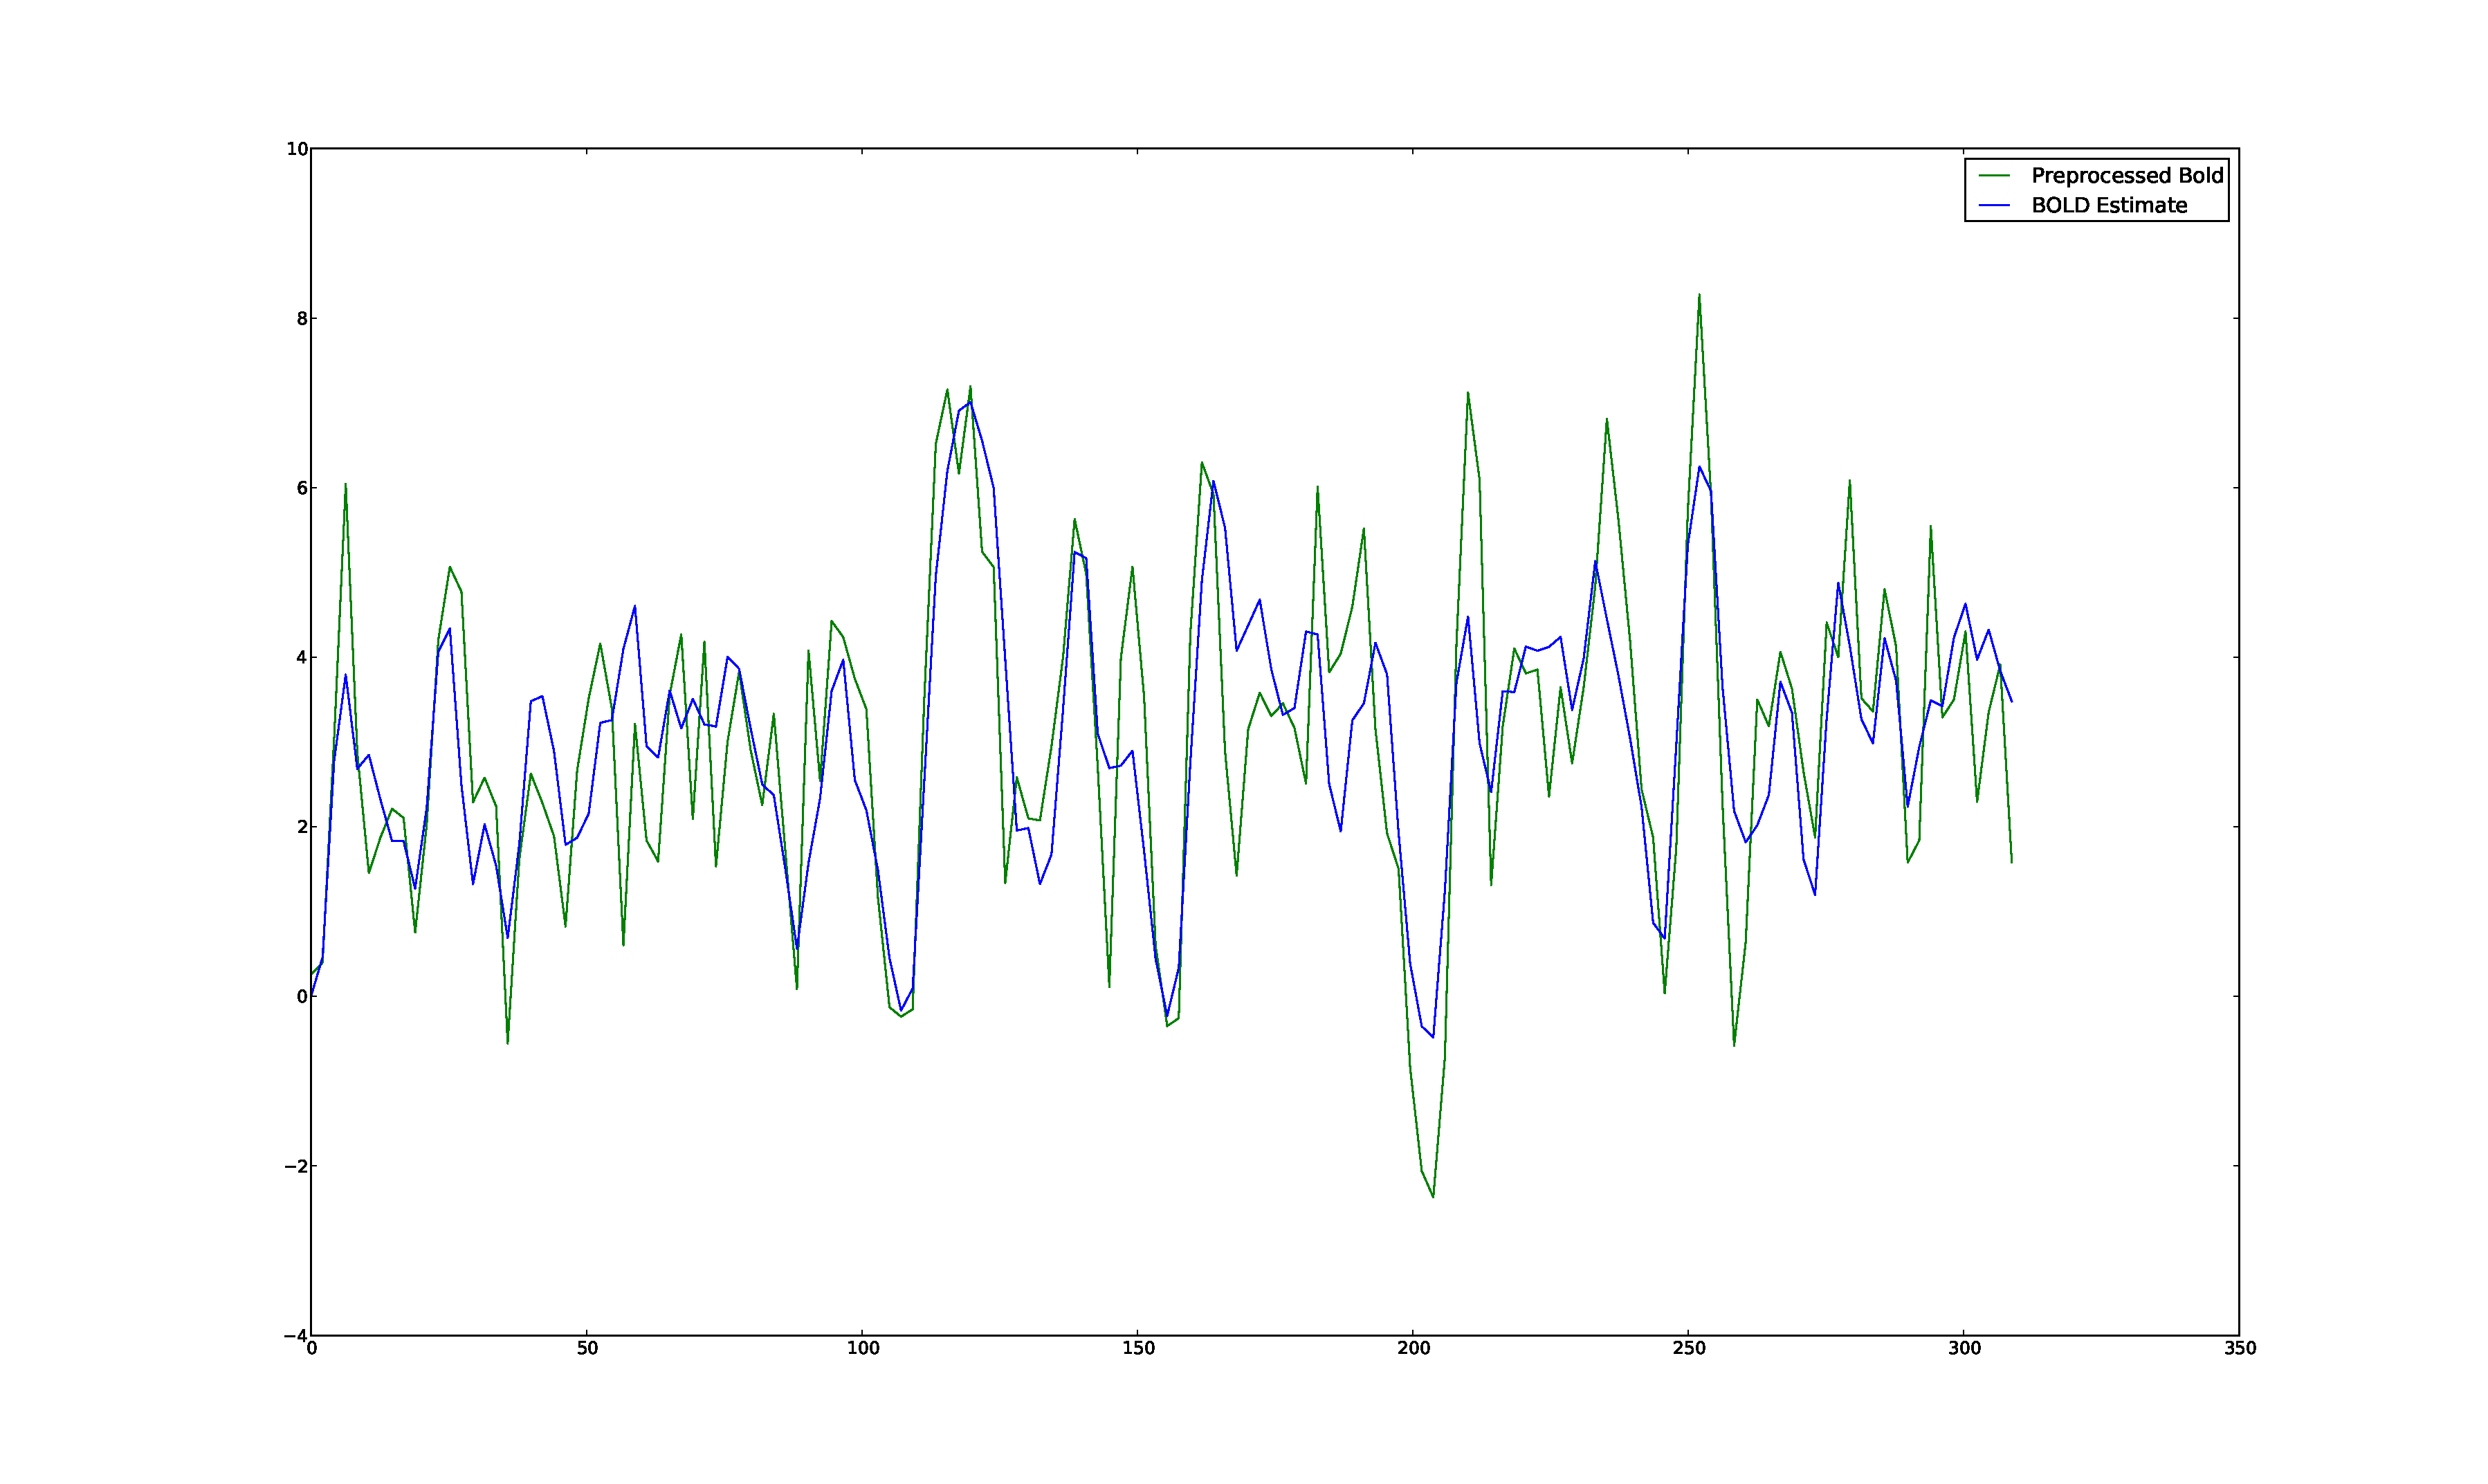
\includegraphics[clip=true,trim=5cm 1cm 4cm 1cm,width=15cm]{images/1_spm_37_14_7}}
\caption{Section 1, Estimated vs. Actual BOLD response}
\label{fig:comp1}
\end{figure}

 
\begin{figure}
\subfigure[Particle Filter]{\label{fig:comp2pfilter} 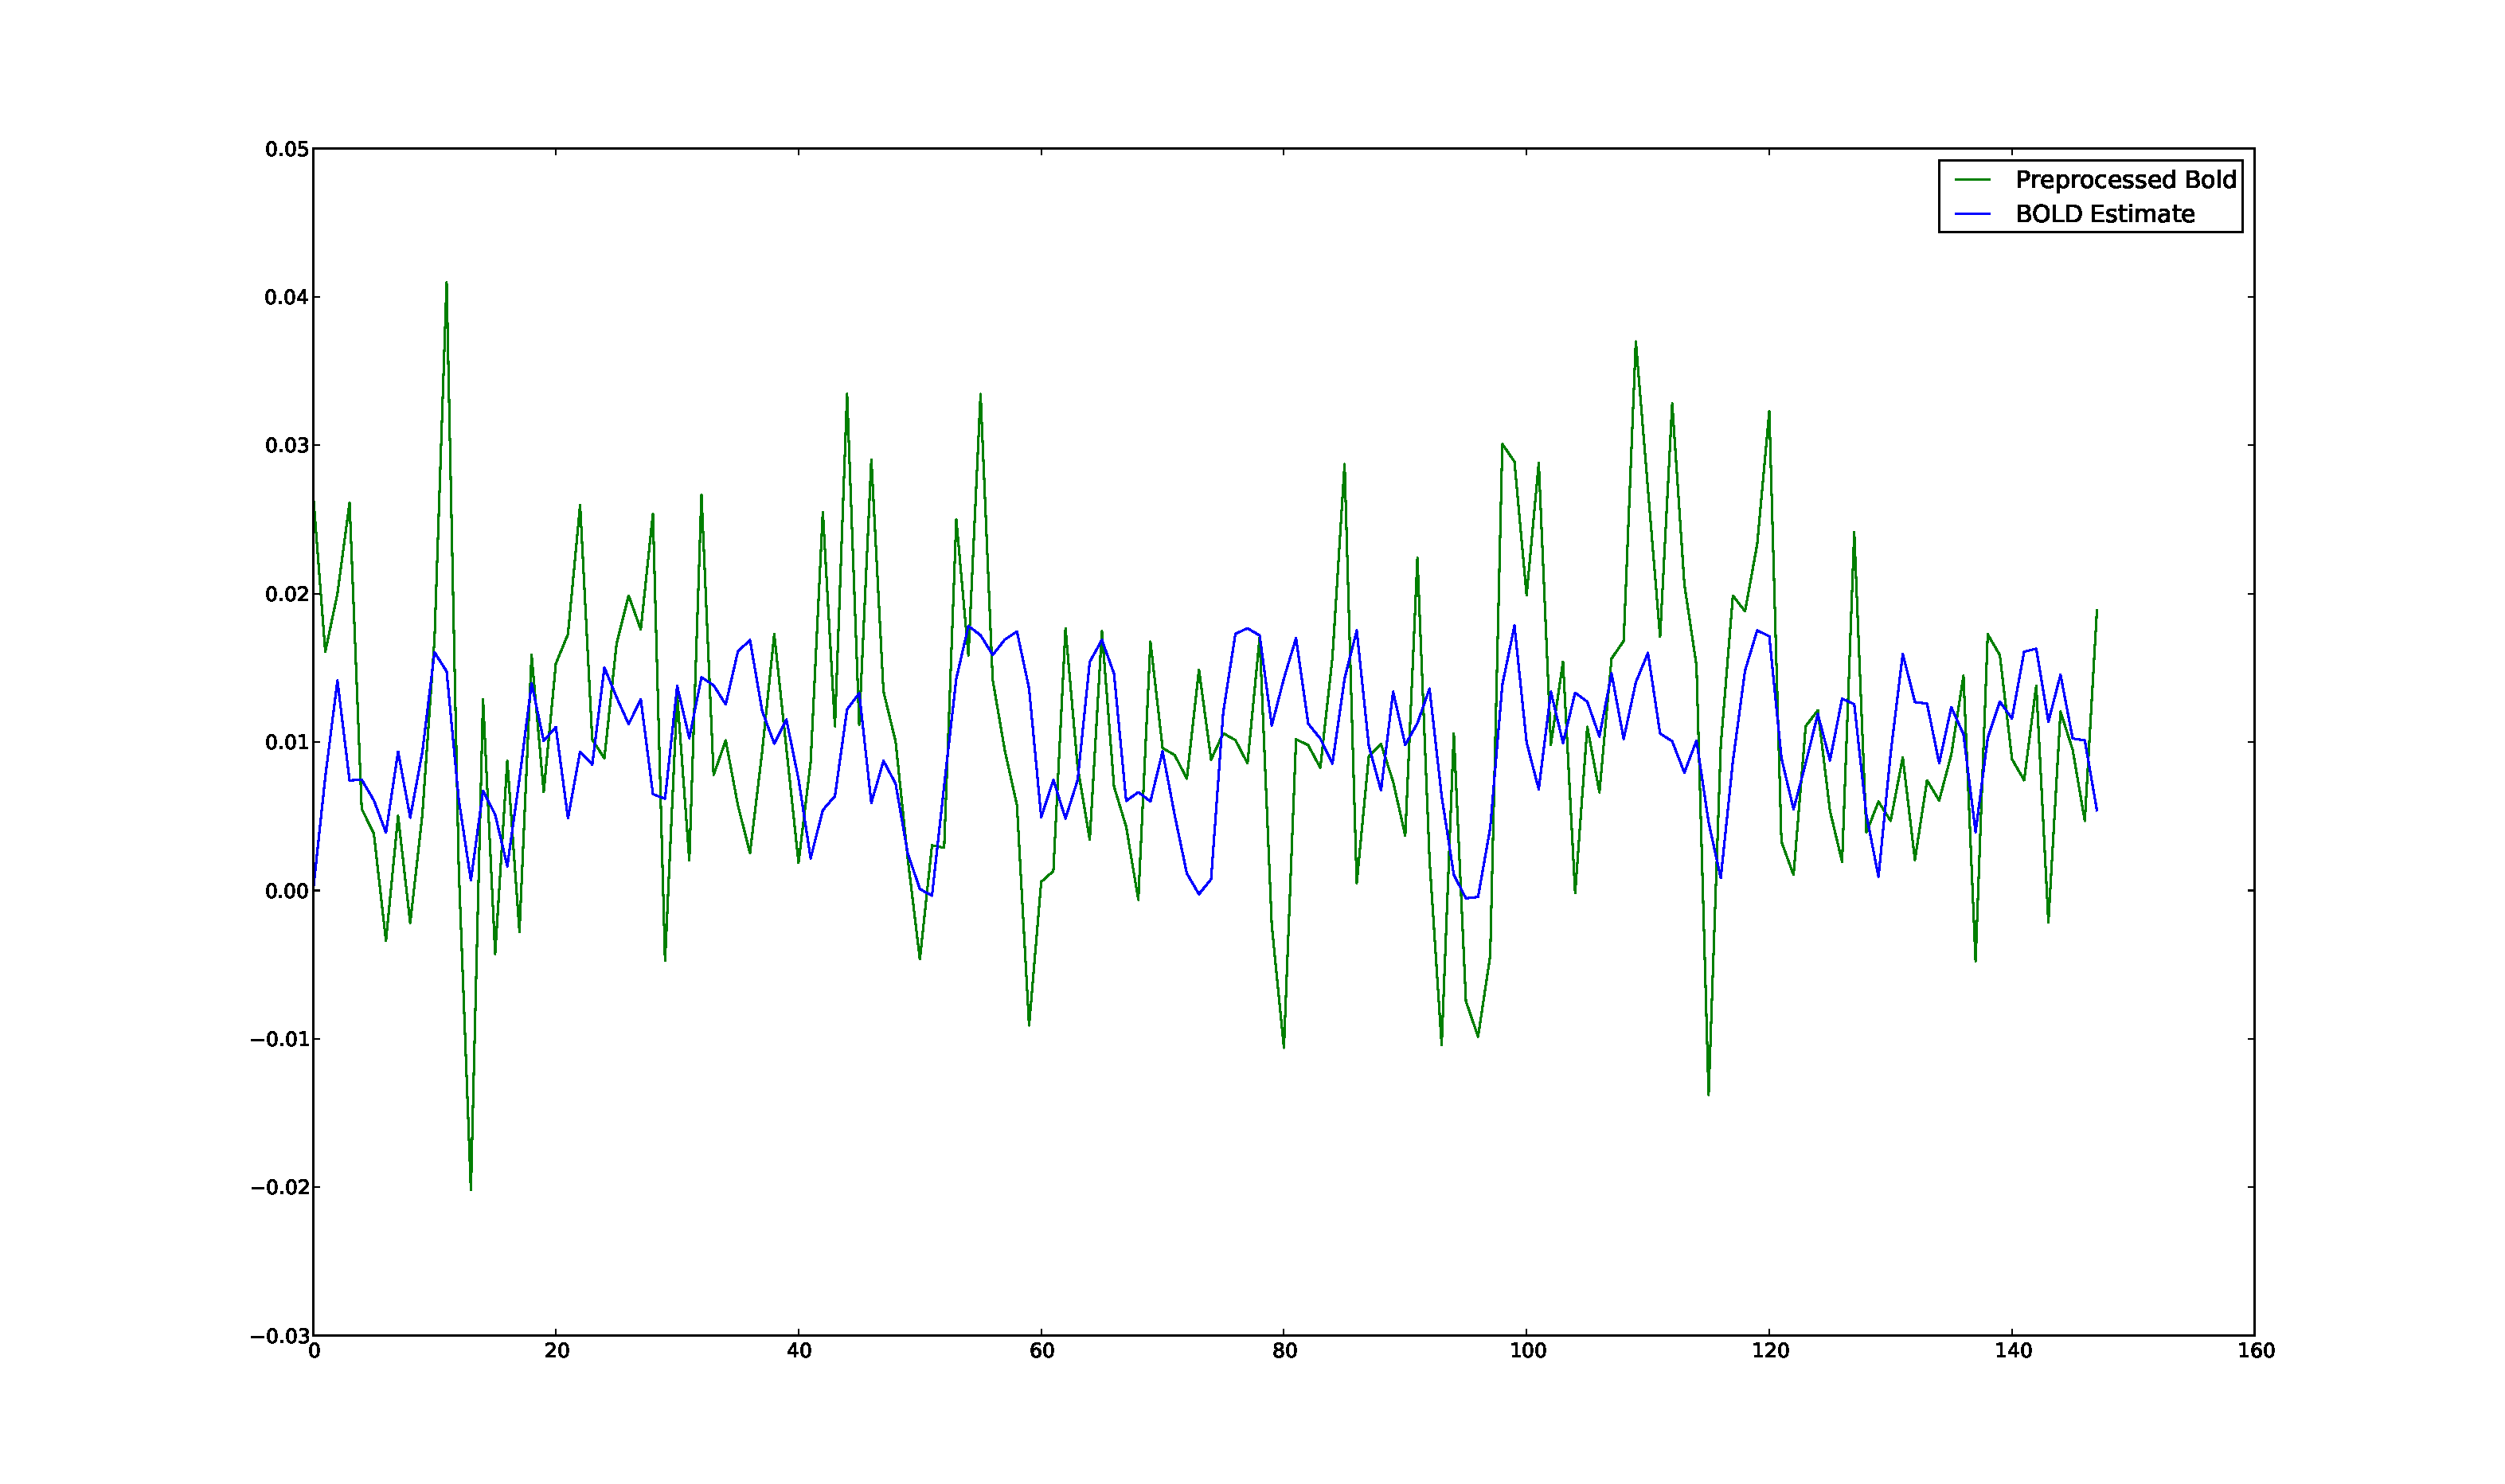
\includegraphics[clip=true,trim=5cm 1cm 4cm 1cm,width=15cm]{images/2_pfilter_34_12_7}}\\
\subfigure[SPM]{\label{fig:comp2spm} 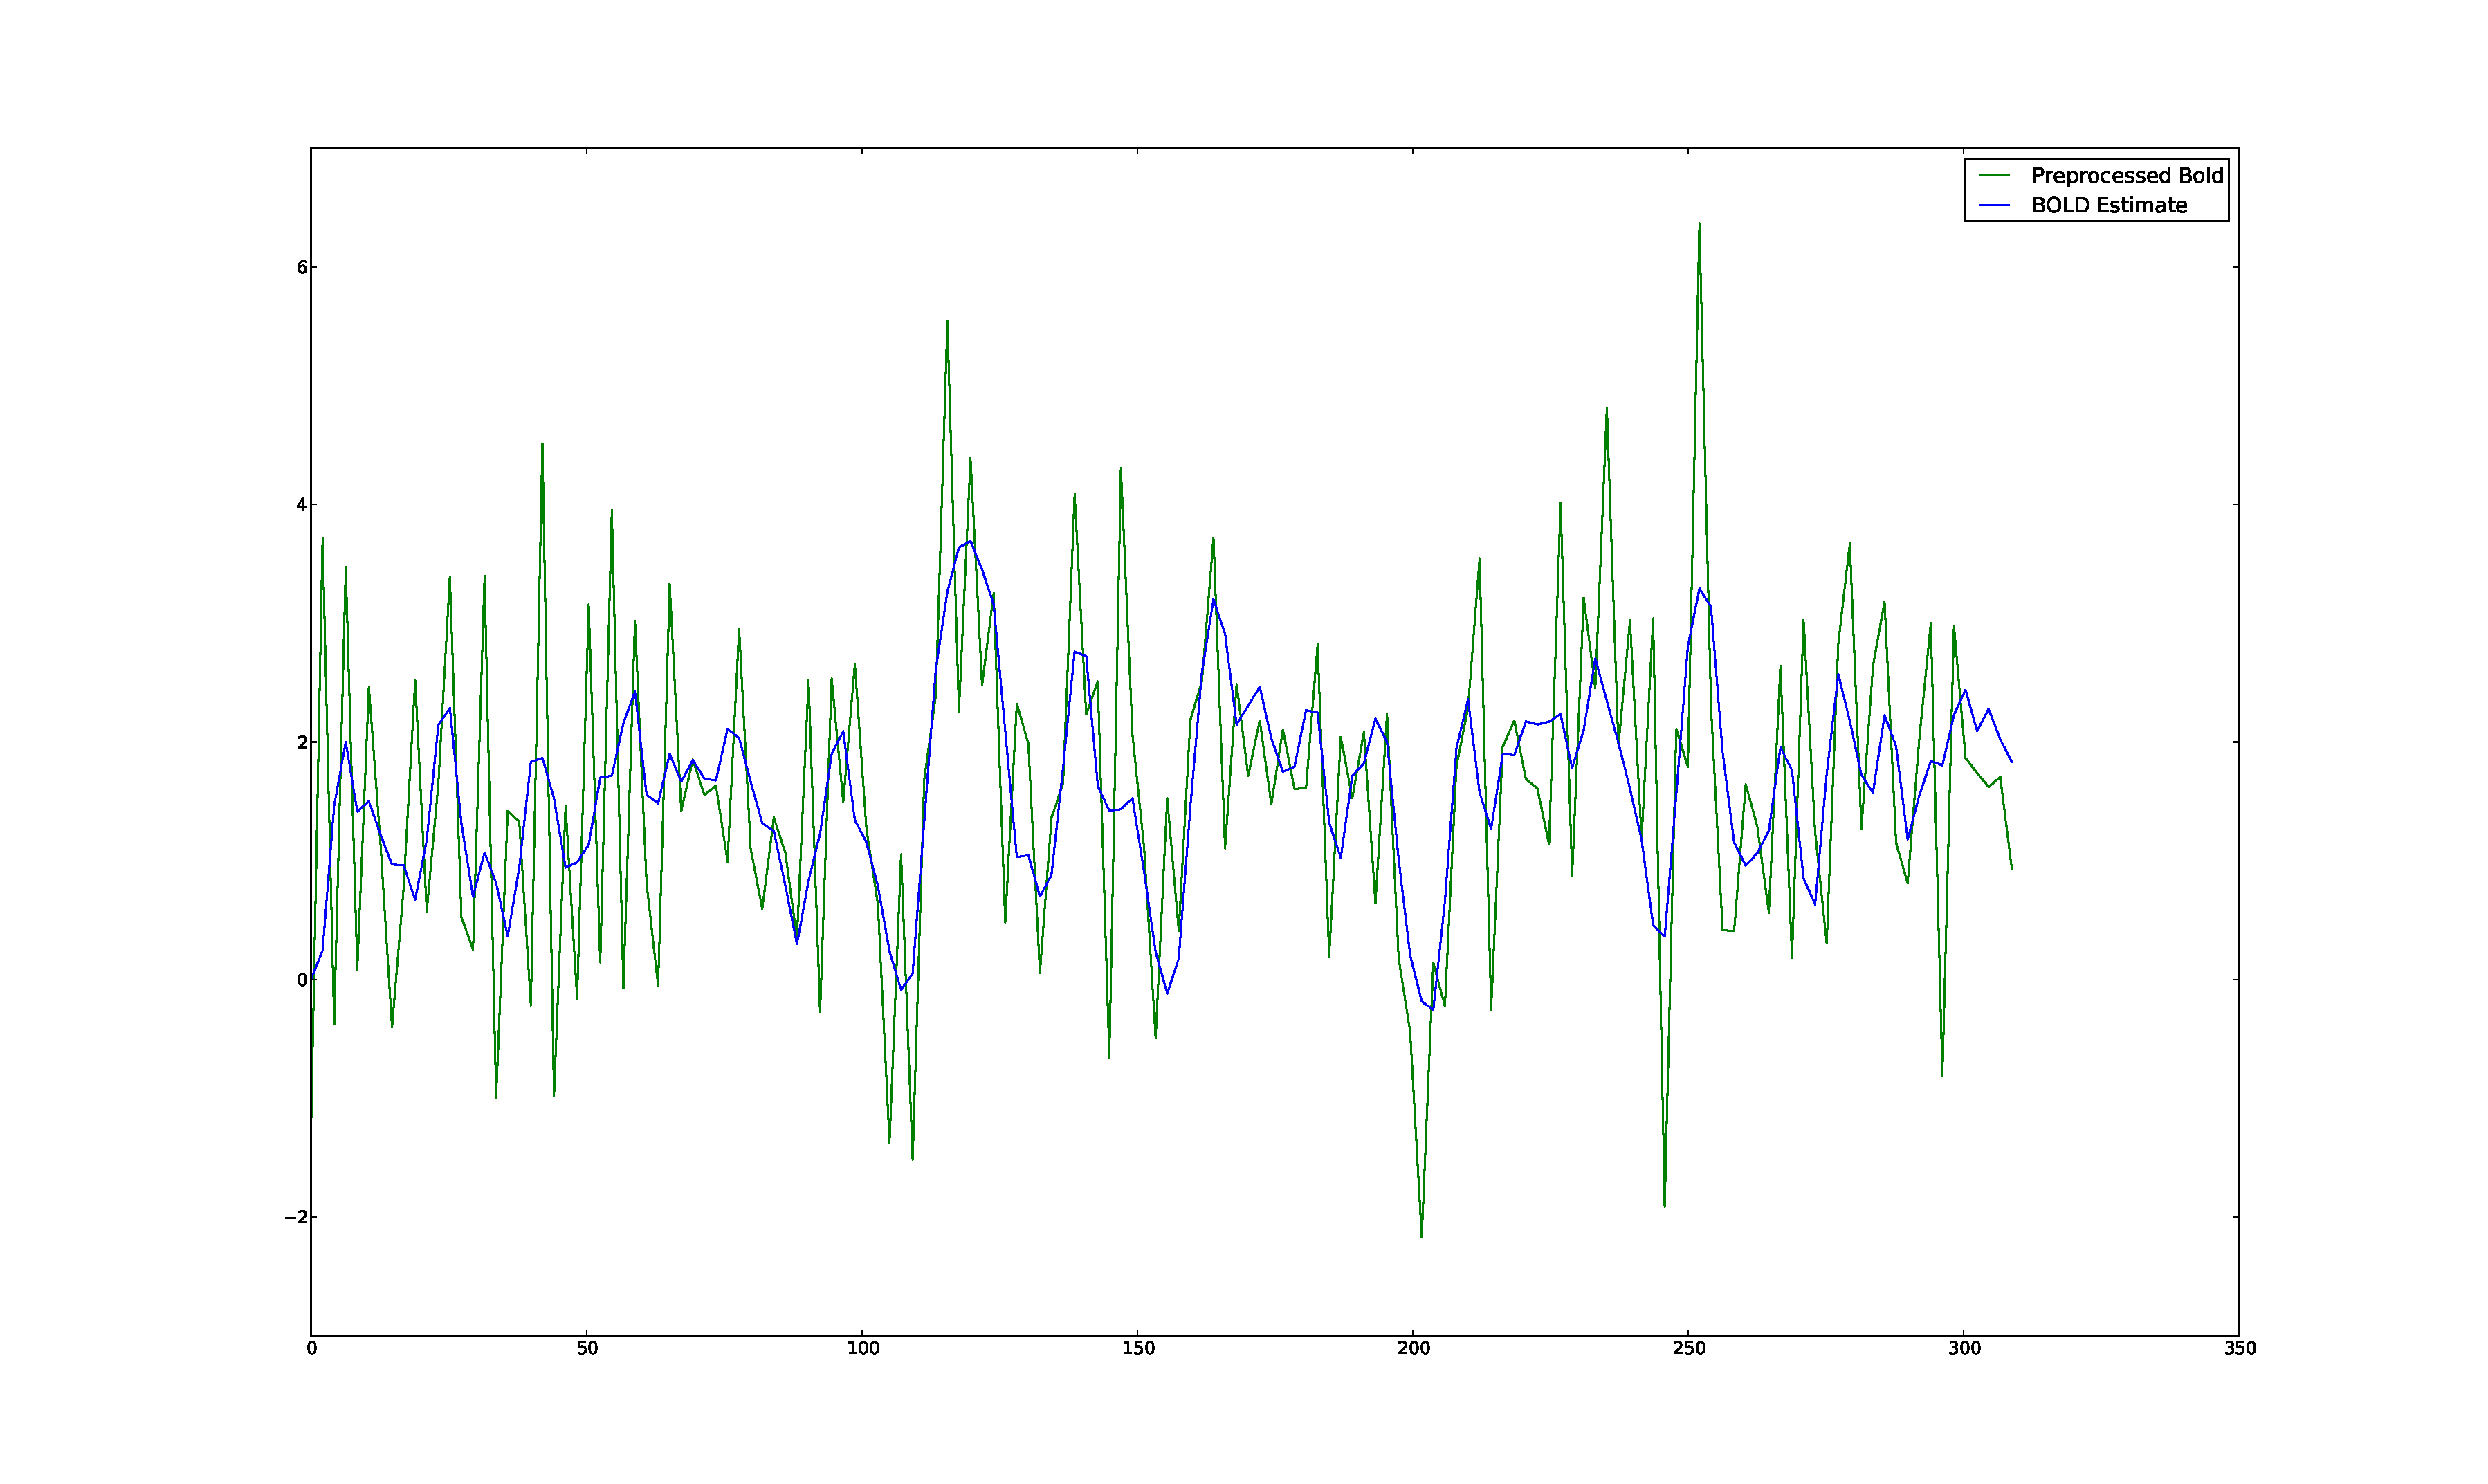
\includegraphics[clip=true,trim=5cm 1cm 4cm 1cm,width=15cm]{images/2_spm_34_12_7}}
\caption{Section 2, Estimated vs. Actual BOLD response}
\label{fig:comp2}
\end{figure}

I chose several voxels to discuss further from \autoref{fig:hm_canon_pfilter} and \autoref{fig:hm_canon_spm}.
The first voxel, labeled 1, had a very high T-score as well as a low error (around $.7$). Thus, the
fit should be very good in both the SPM and particle filter output; this comparison is shown in 
\autoref{fig:comp1}. Recall that SPM worked on a slightly less noisy time series because of the
spatial smoothing; this explains the lack of the sharp peak in the particle filter's preprocessed
data. Regardless, as expected, both fits are very good.

I chose the second voxel (\autoref{fig:comp2}) because it was active in SPM and it would appear to be in a prime
location to be active in the SPM image (given the results in the surrounding voxels). The fit,
however shows just why the voxel did not have a particularly good error. Although certain peaks 
seem to fit rather well the input doesn't seem to correlate that well with the BOLD response. For
instance 75 seconds in, the stimulus is clearly not present, and so the signal should drop off; yet
it doesn't. This is a good example of a voxel that seems to be reacting to something in addition to
the direct stimulus. Even in what should be a rather smooth time-series in SPM, the BOLD signal
looks very noisy. 

The third voxel, compared in \autoref{fig:comp3}, was far away from any other active voxels 
and yet had a very low (around $.7$) residual.
In both preprocessed time-series the input is extremely noisy, yet by the normalized residual 
the response is good. This could be an example of a false positive, although the general trend
of the response seems to follow the estimated response. 

Whereas the third voxel was a region that was considered active by the particle filter
algorithm but not SPM; the fourth voxel is the reverse. The particle filter did not
find a good fit, but in SPM8 the voxel had a decently high T-score. \autoref{fig:comp4} shows
the line fit for each algorithm, and neither are particularly good; though in a few areas
the upward or downward movements seem to be correlated. Regardless, this would seem to be
a false positive from SPM8. 

The fifth, and last single voxel to be analyzed is one more area that had a low residual according
to the particle filter, and yet did not show up in SPM. The line fit is shown in \autoref{fig:comp5},
and unlike voxel 3 is certainly \emph{not} a false positive. Regions such as this are a very 
good example of why spatial smoothing can be problematic. By having a more adaptive model, and
thus reducing bias error, it is possible to get a very good fit to single voxels such as this,
and thus the need for spatial smoothing is somewhat reduced. 

\begin{figure}
\subfigure[Particle Filter]{\label{fig:comp3pfilter} 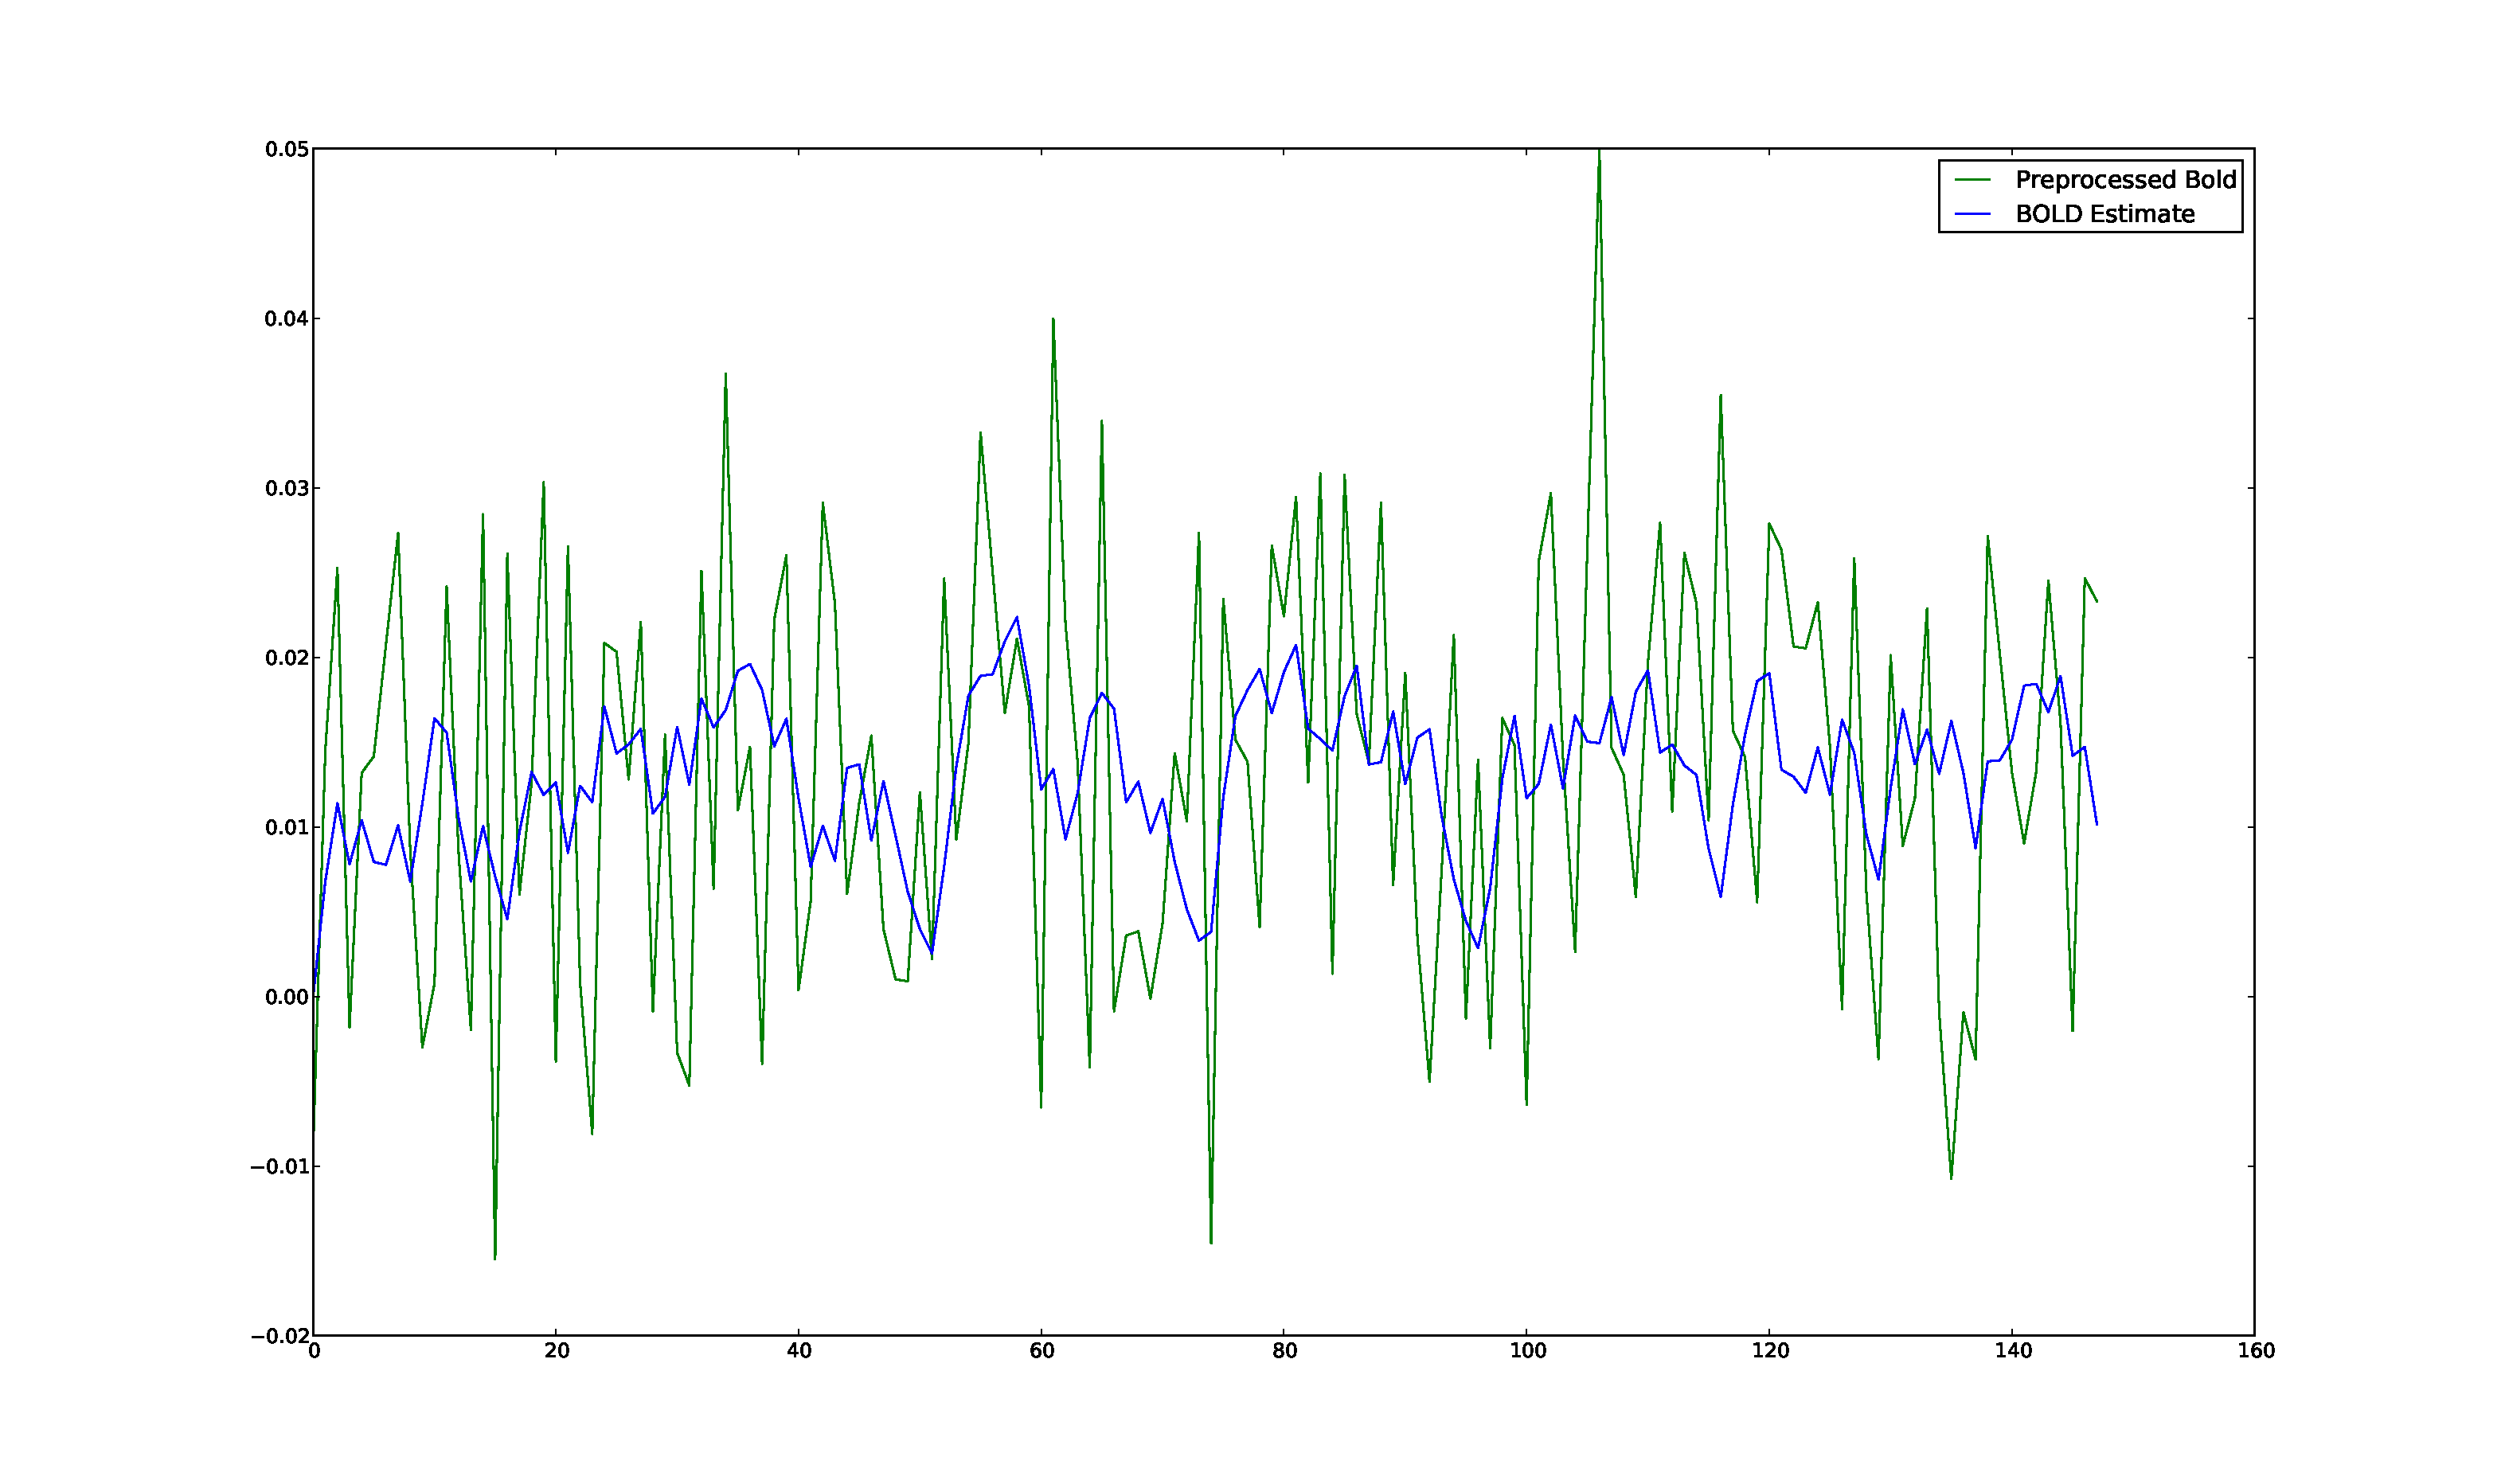
\includegraphics[clip=true,trim=5cm 1cm 4cm 1cm,width=15cm]{images/3_pfilter_23_21_7}}\\
\subfigure[SPM]{\label{fig:comp3spm} 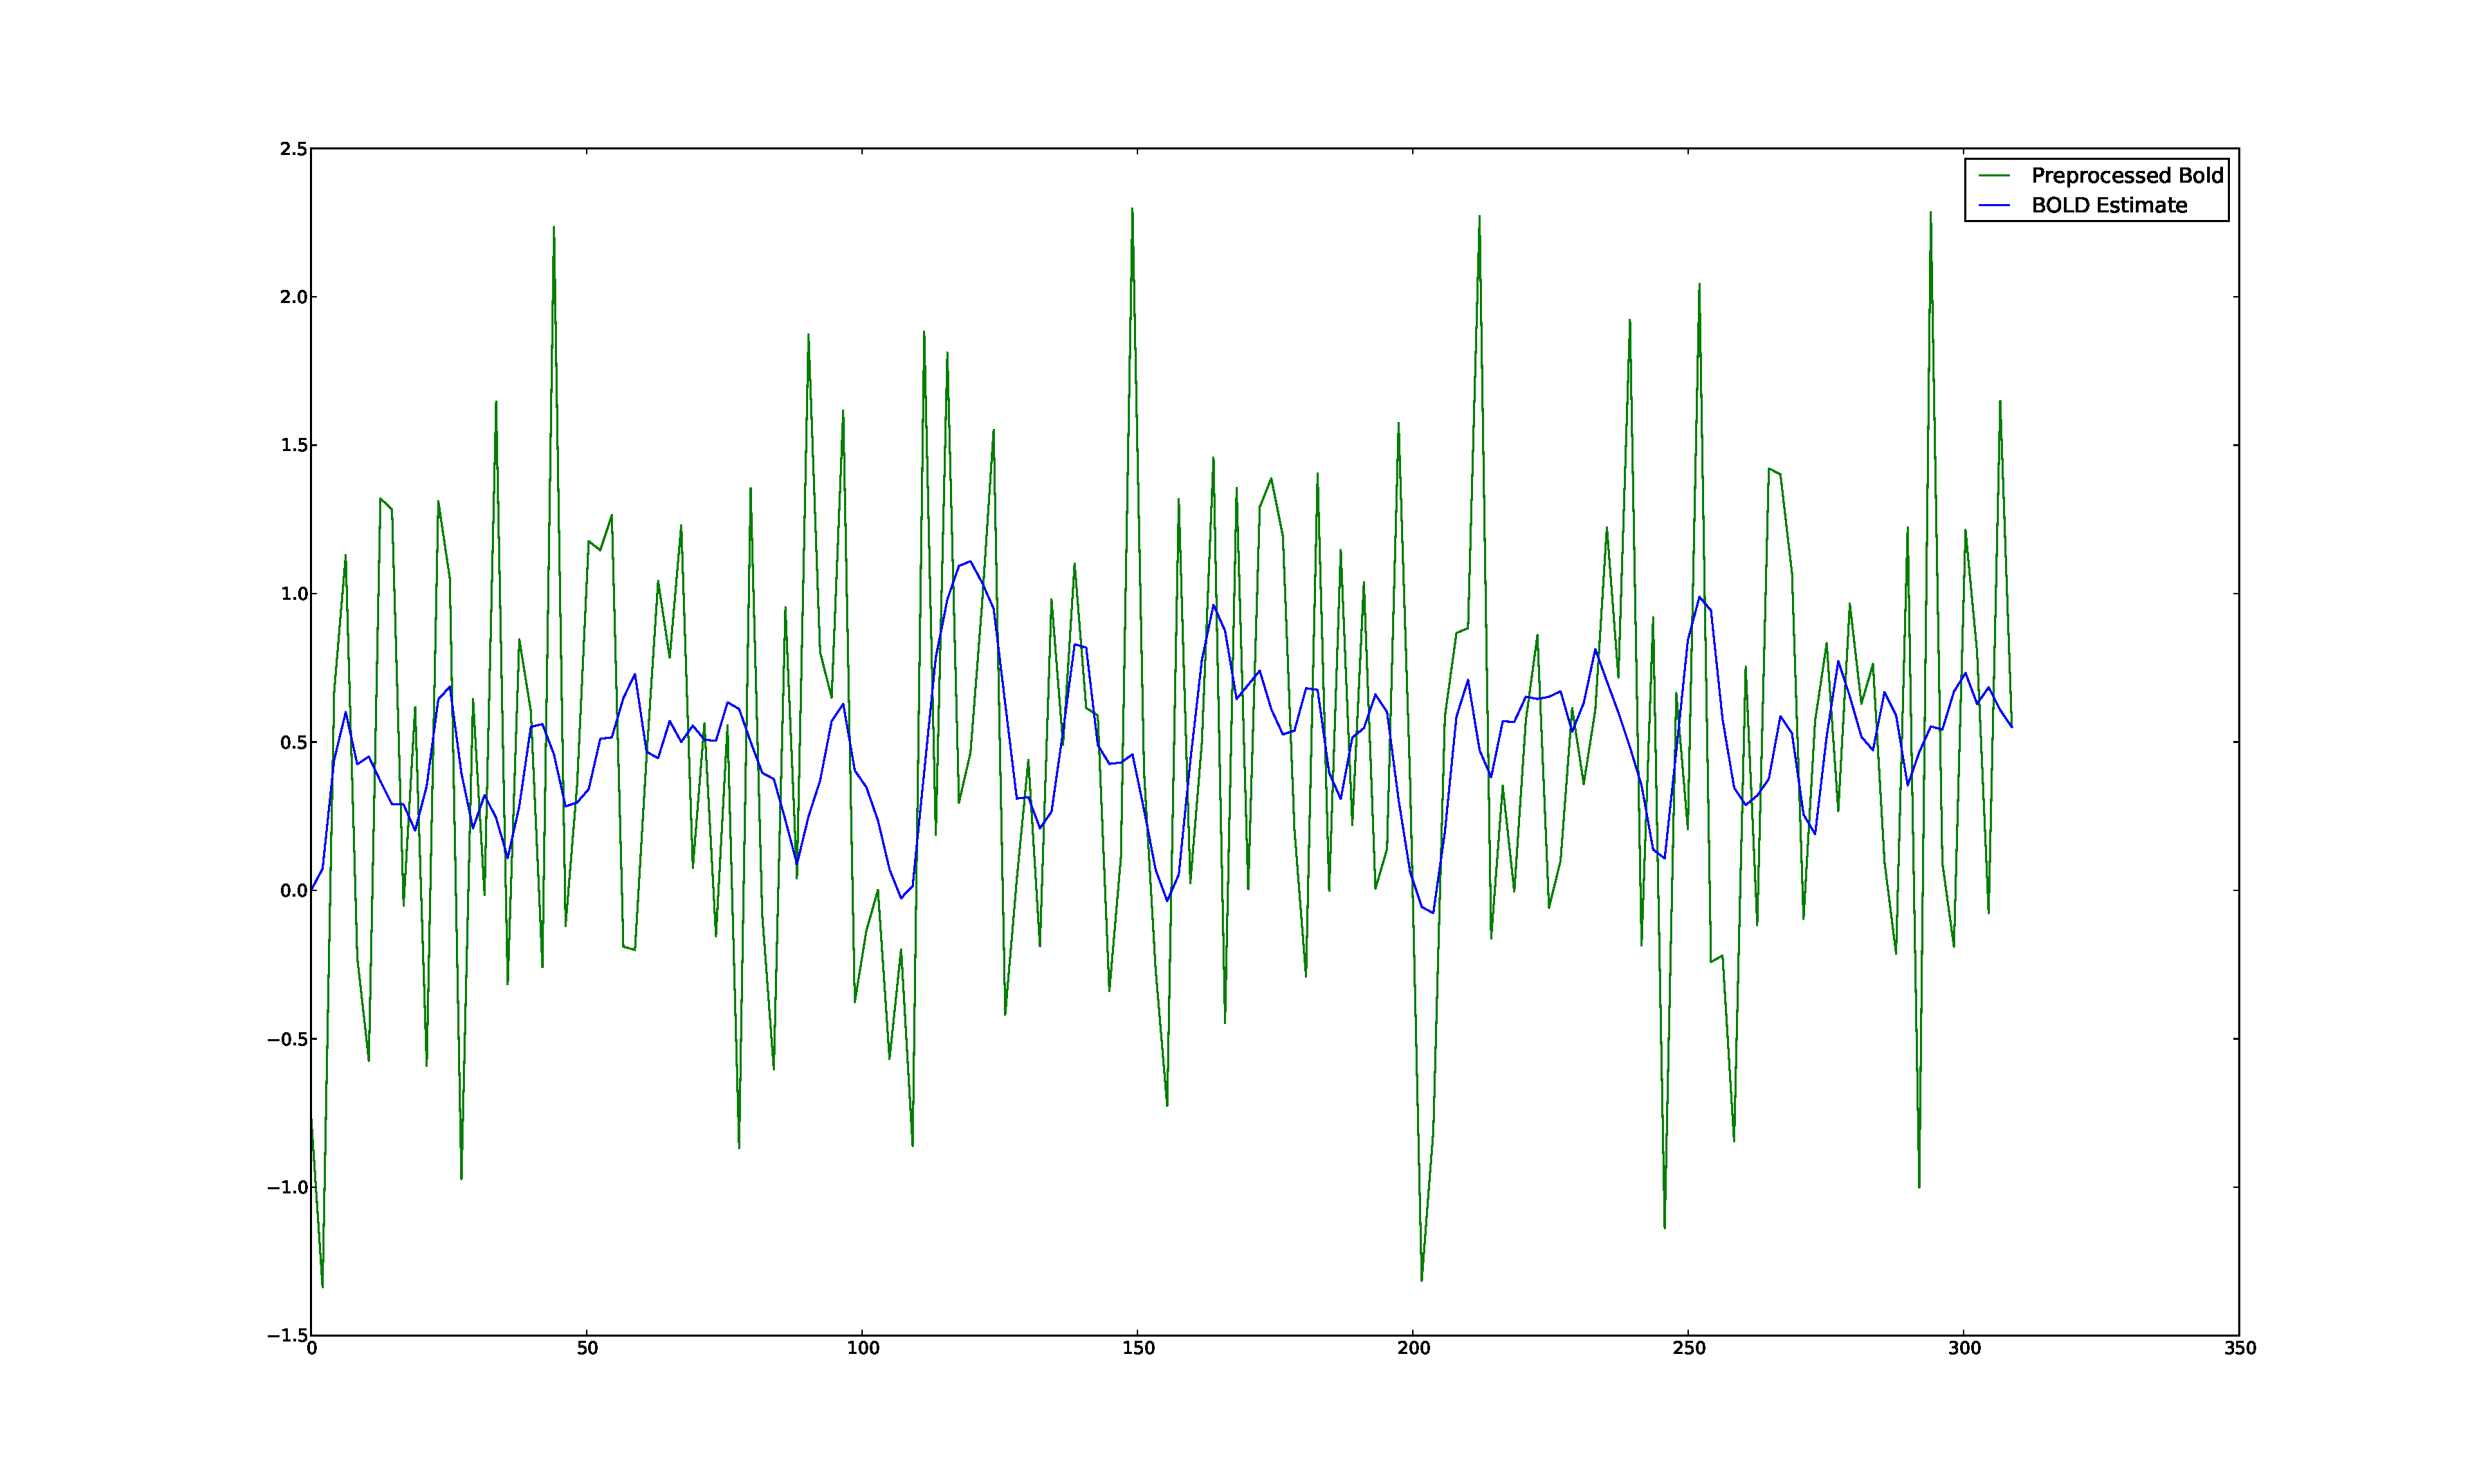
\includegraphics[clip=true,trim=5cm 1cm 4cm 1cm,width=15cm]{images/3_spm_23_21_7}}
\caption{Section 3, Estimated vs. Actual BOLD response}
\label{fig:comp3}
\end{figure}

\begin{figure}[H]
\subfigure[Particle Filter]{\label{fig:comp4pfilter} 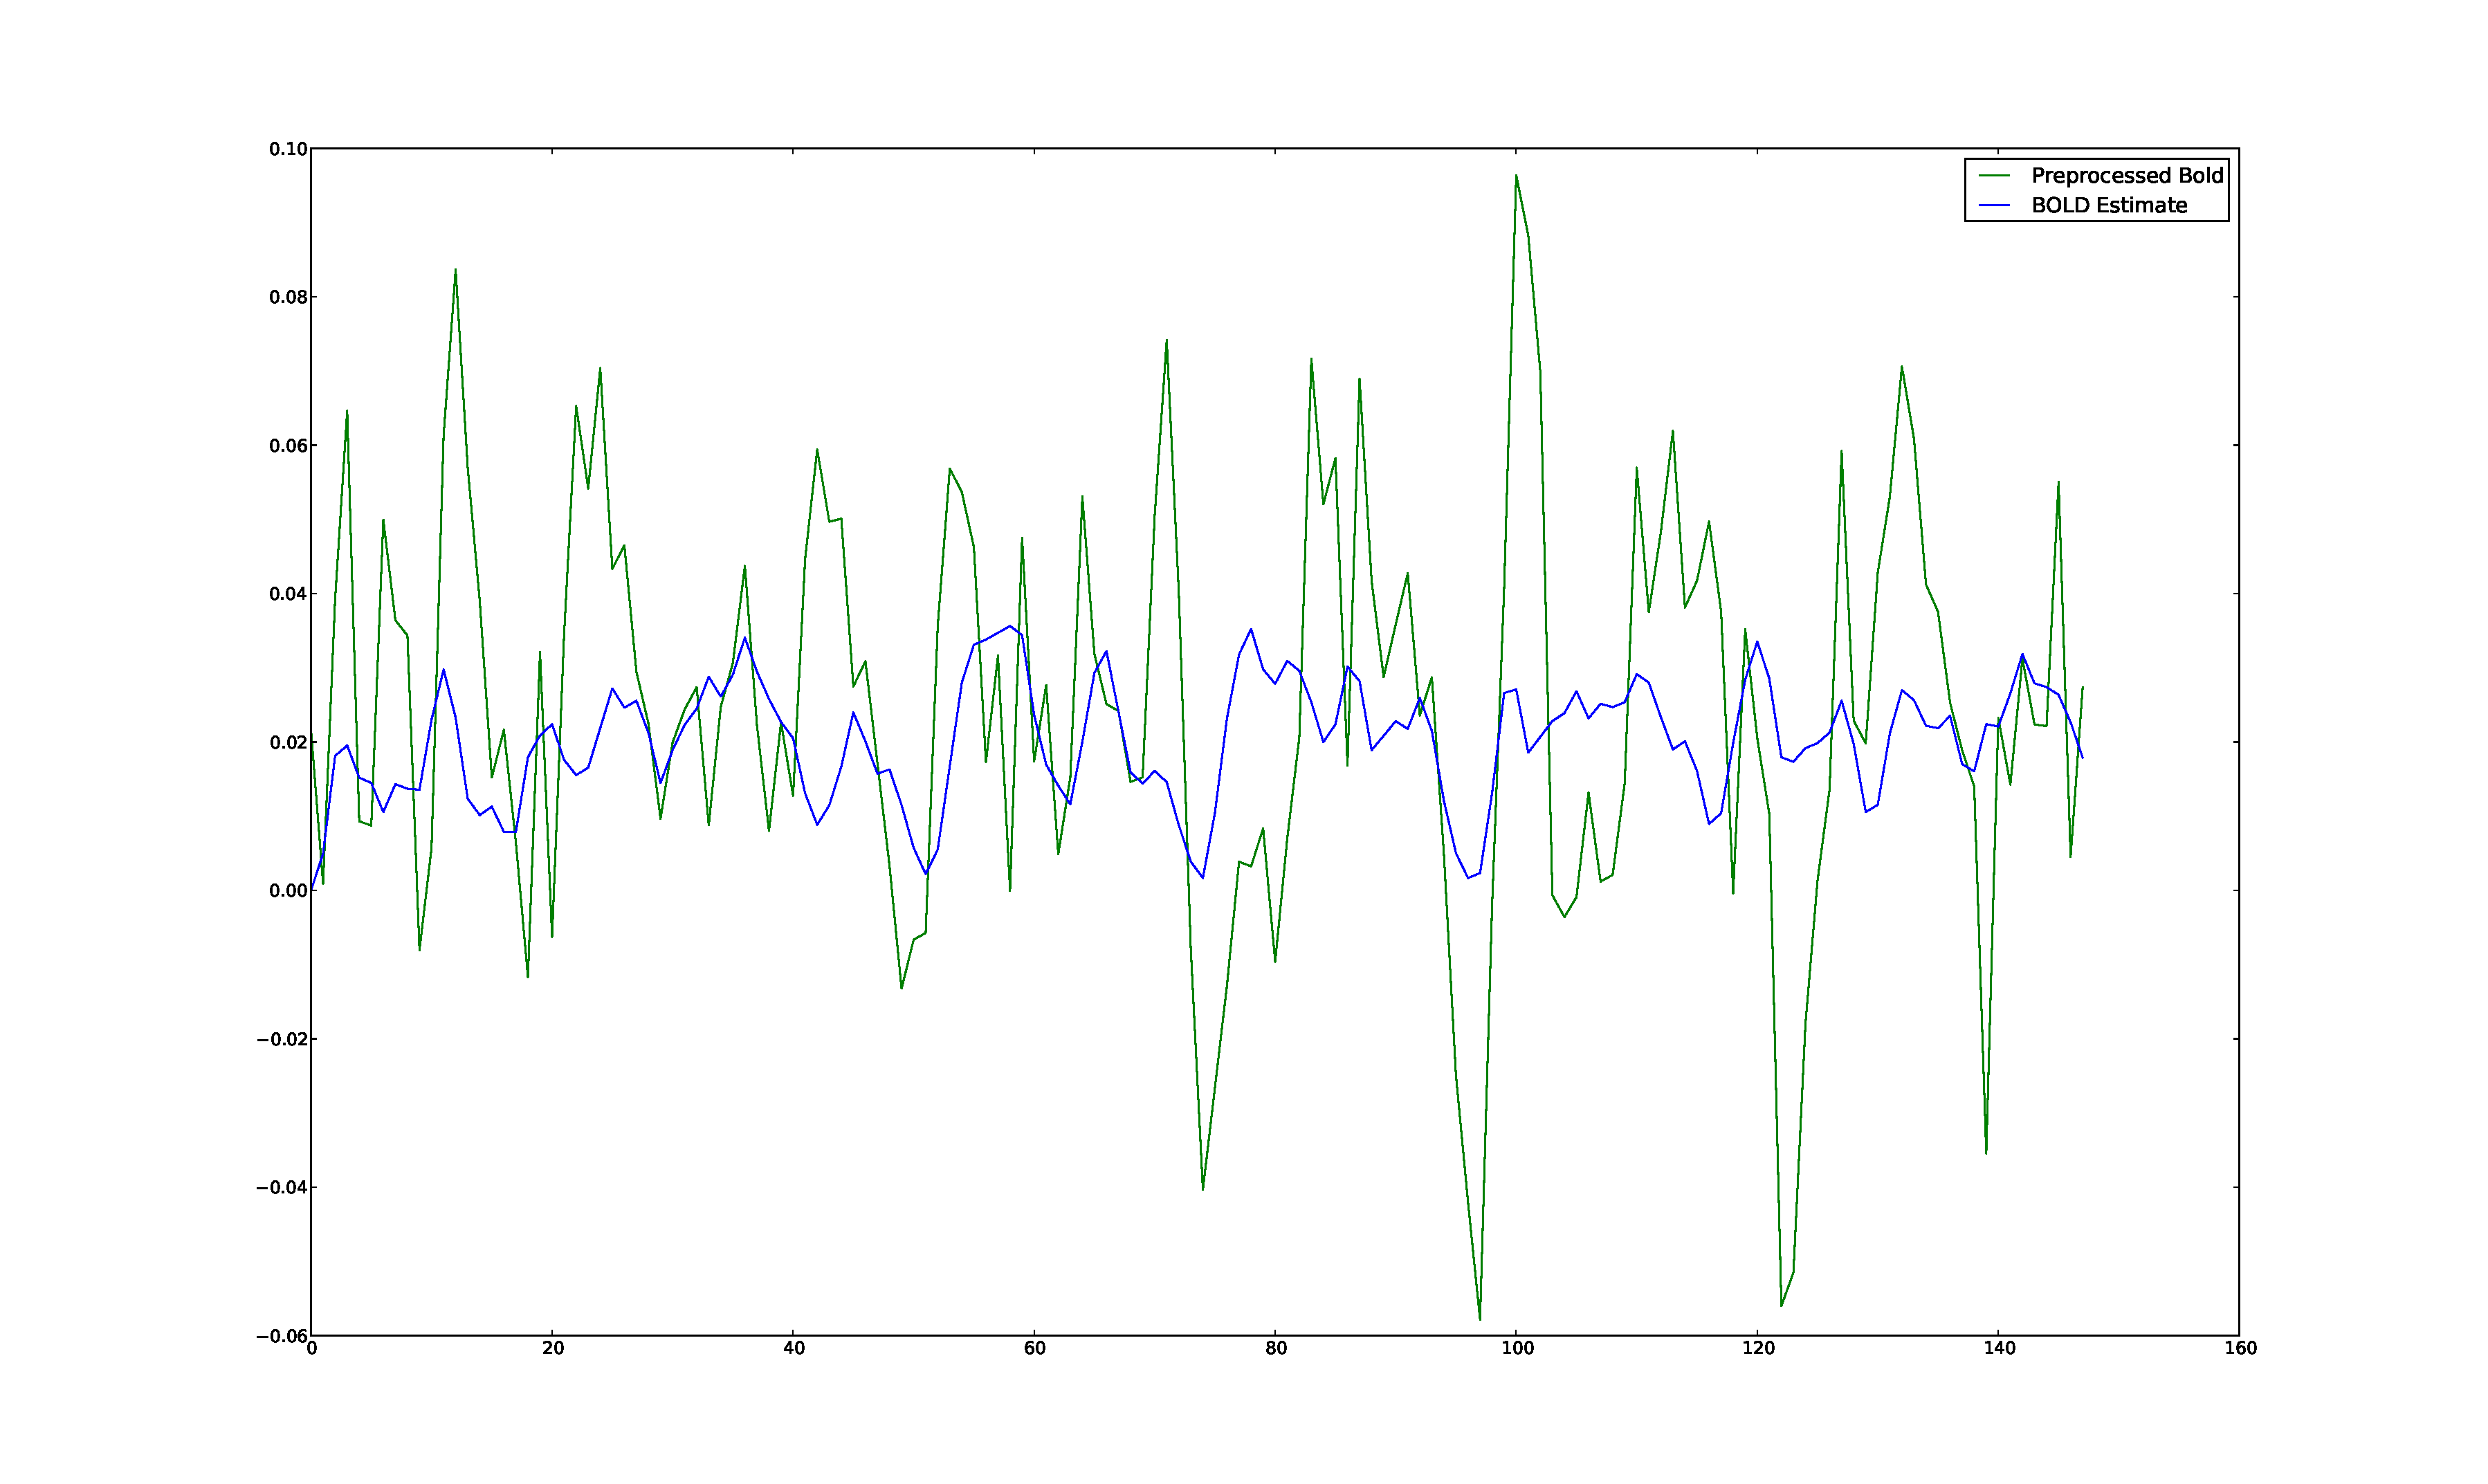
\includegraphics[clip=true,trim=5cm 1cm 4cm 1cm,width=15cm]{images/4_pfilter_26_15_7}}\\
\subfigure[SPM]{\label{fig:comp4spm} 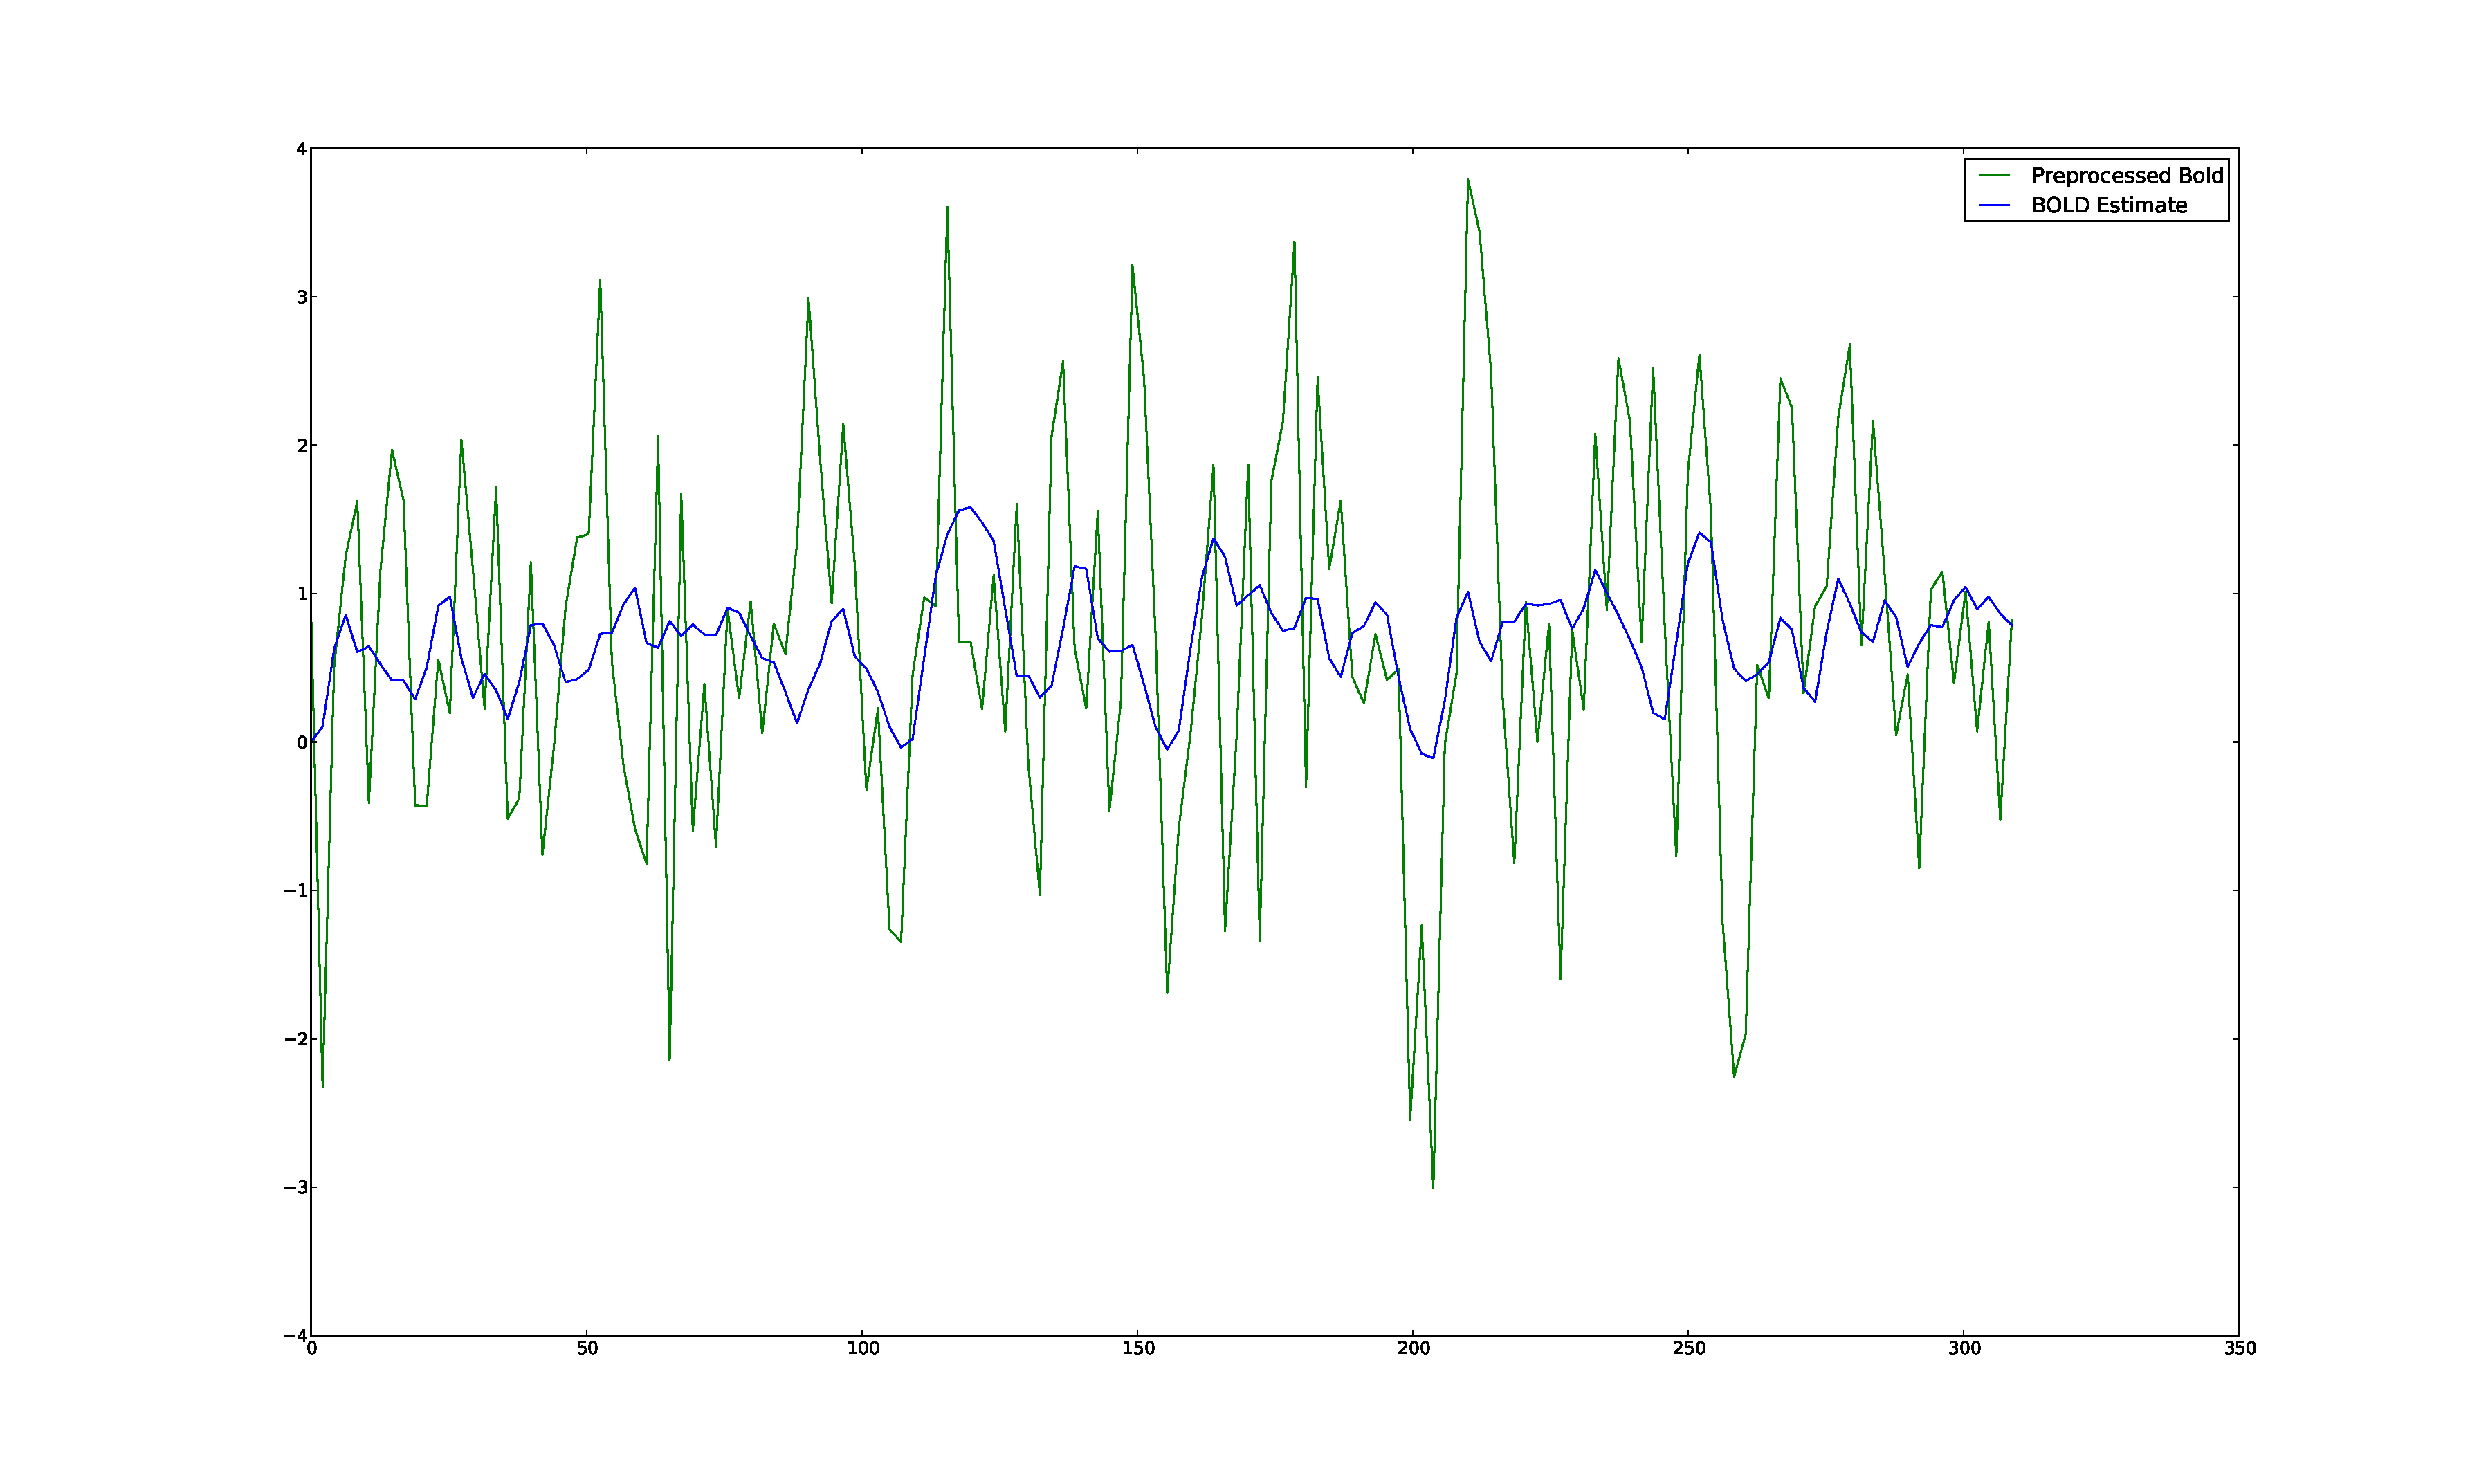
\includegraphics[clip=true,trim=5cm 1cm 4cm 1cm,width=15cm]{images/4_spm_26_15_7}}
\caption{Section 4, Estimated vs. Actual BOLD response}
\label{fig:comp4}
\end{figure}

\begin{figure}
\subfigure[Particle Filter]{\label{fig:comp5pfilter} 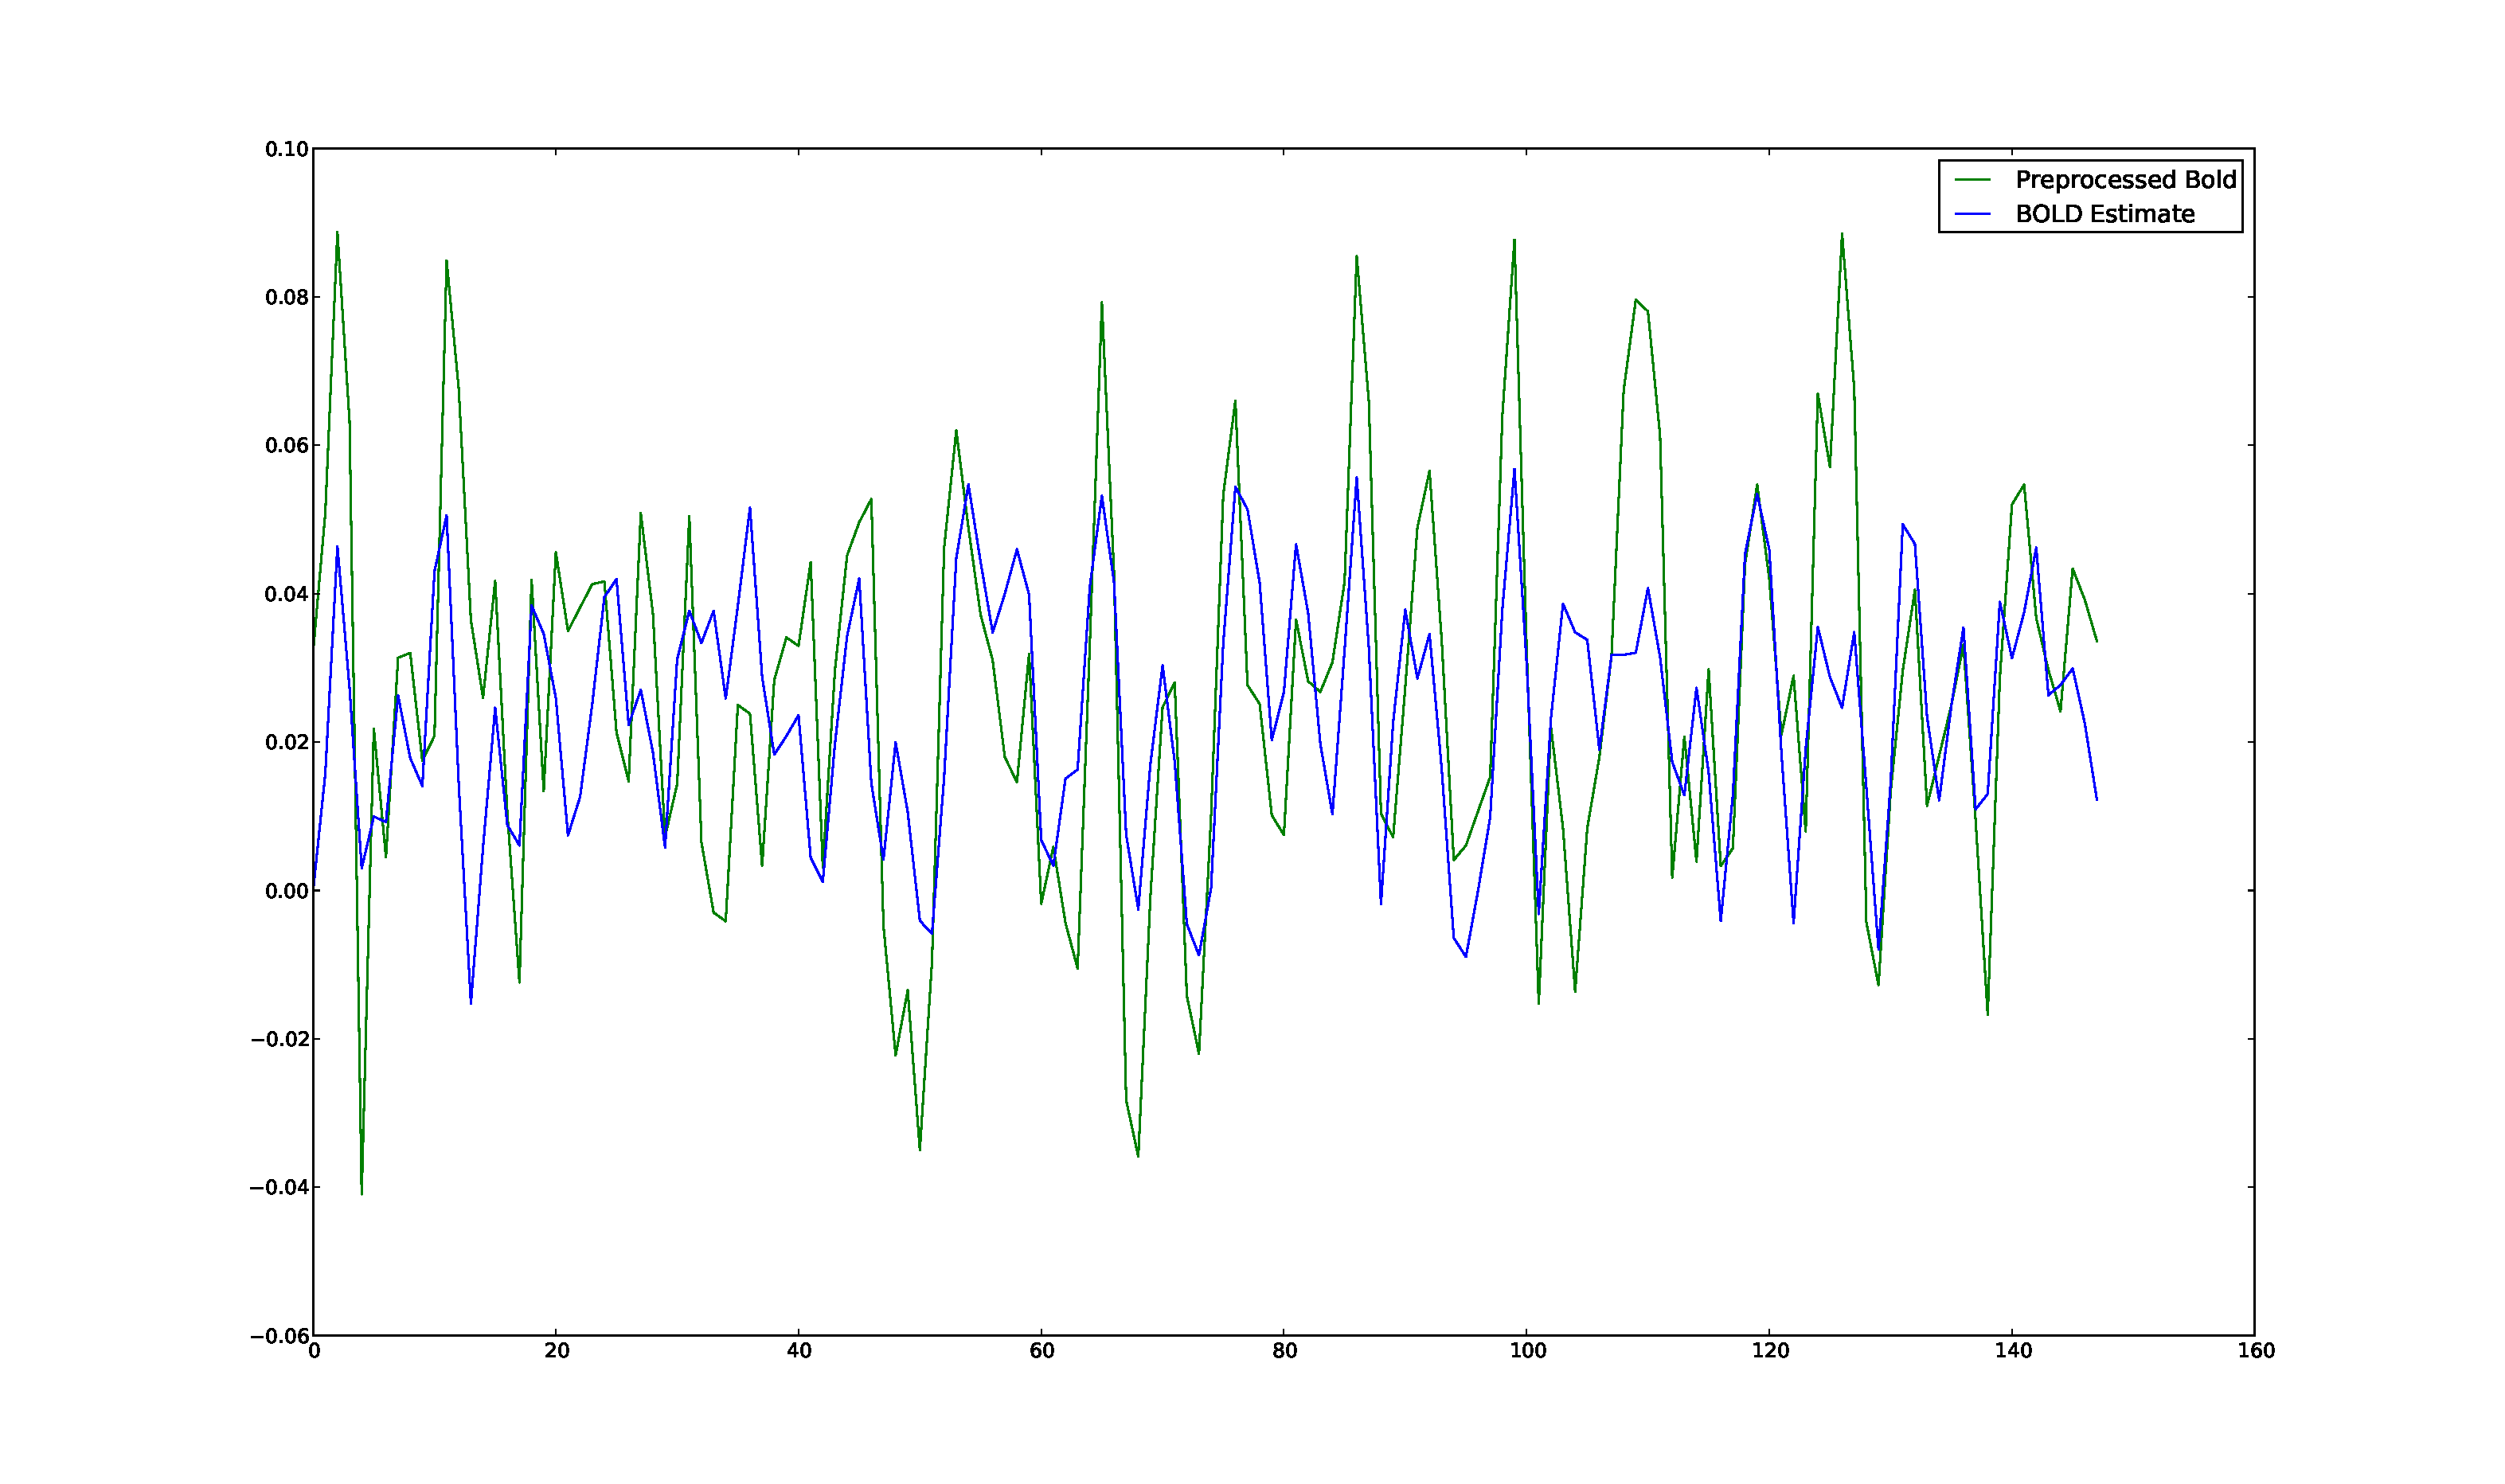
\includegraphics[clip=true,trim=5cm 1cm 4cm 1cm,width=15cm]{images/5_pfilter_25_34_25}}\\
\subfigure[SPM]{\label{fig:comp5spm} 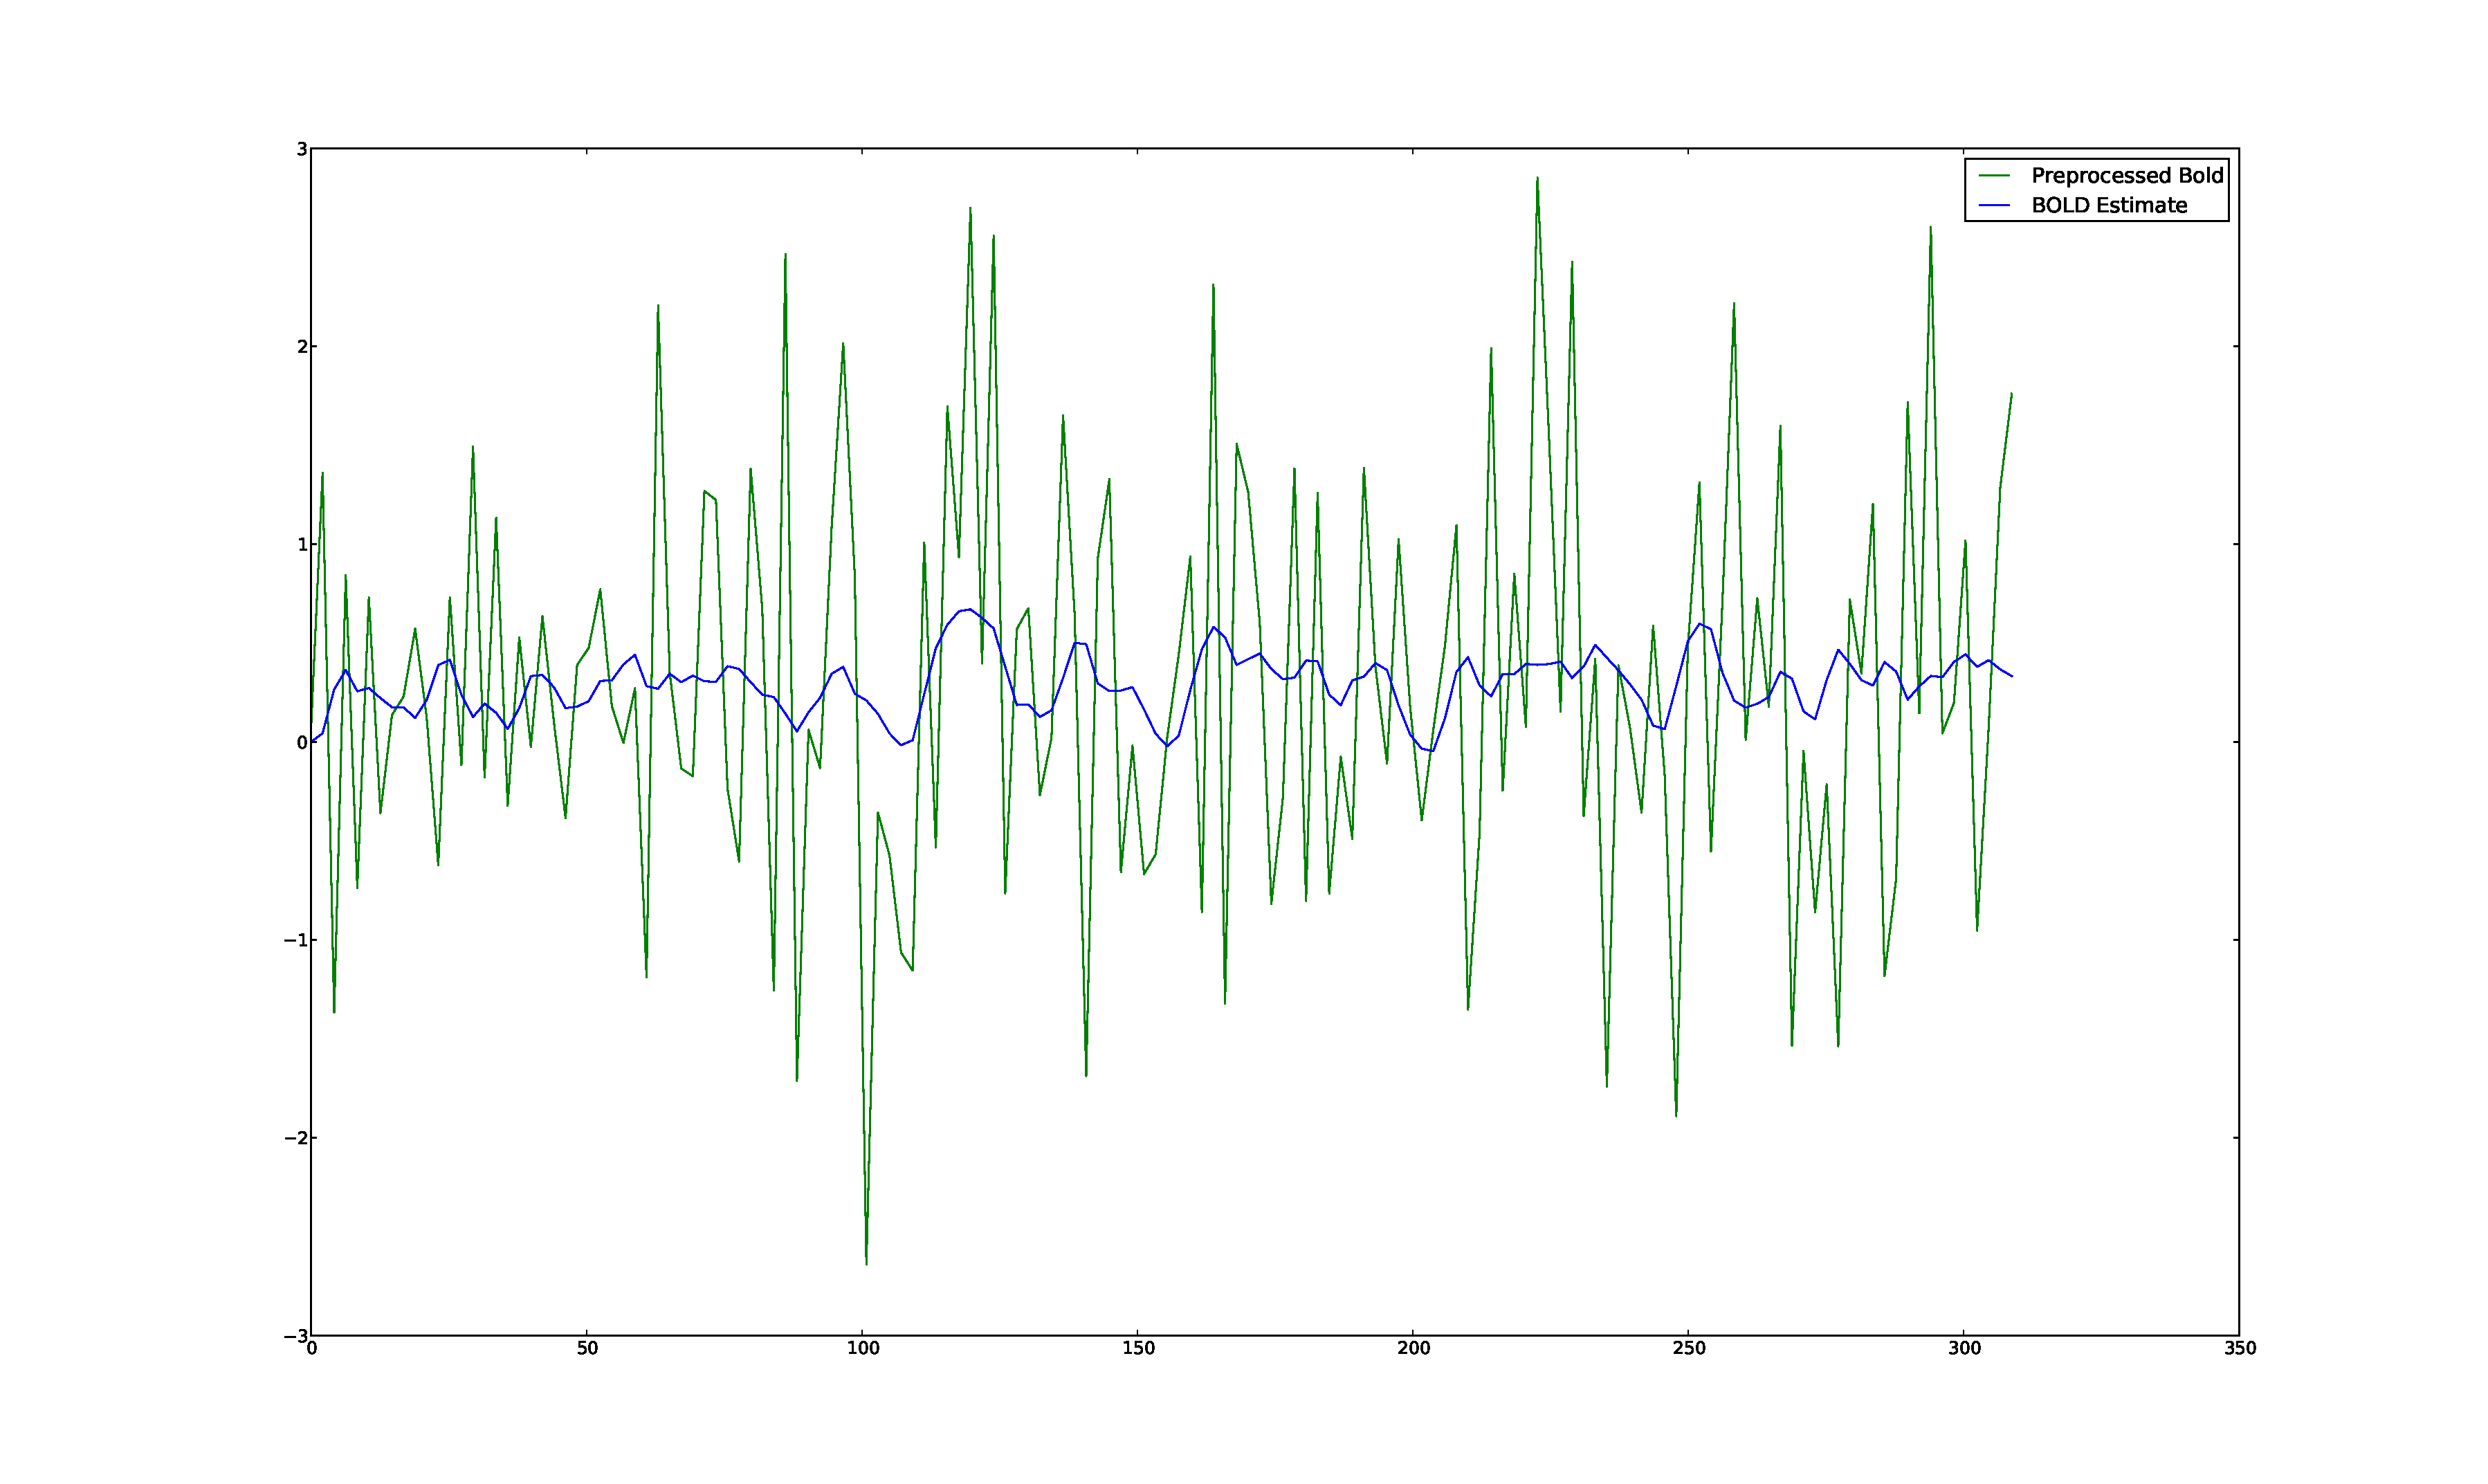
\includegraphics[clip=true,trim=5cm 1cm 4cm 1cm,width=15cm]{images/5_spm_25_34_25}}
\caption{Section 5, Estimated vs. Actual BOLD response}
\label{fig:comp5}
\end{figure}

\section{Discussion}
From the maps generated, the similarities to SPM8's results are encouraging. At the 
very least the output of the particle filter seems to meet the quality of SPM. The normalization
of the residual is certainly necessary. Although there is no hard threshold on the 
normalized residual, it would appear that the normalization is providing a reasonable
ordering of regression quality. The question of what threshold to use is a difficult one.
The actual division of the residual by an estimate for the standard deviation
of the signal would seem to mandate a threshold less than one. However, recall that the 
same media-absolute-deviation was added to the de-trended signal as a DC-gain. This means
that a flat, no-response bold signal will actually have a residual greater than the standard 
deviation of the signal. Then again, the residual may be reduced for any point where the 
model spikes up due to stimuli. Ultimately if the model were to run right down the 
center of the distribution the residual would be equal to the MAD, and would have a 
normalized residual of 1. Thus, again, a normalized residual of 1 is at least as 
good as a flat line at the median. 
Other measures of fitness could also be used such as mean of the absolute error or 
mutual information. Although least squares is the best linear unbiased estimator,
this signal is heavily nonlinear, so other estimators may exceed the OLS in terms
of likelihood. Regardless, the normalized residual provides a good solution at this
point, comparable to SPM.
